\chapter{Interference}
% Lesson Six: Interference

In this chapter, we will talk about one of the most fundamental phenomena concerning waves: interference. We will start by considering interference with normal single frequency waves when they superpose. Then we will move to interference of single photons, and we will conclude with interference of qubits.

\section{Constructive and destructive interference}


% Step One: Constructive and Destructive Interference

Let's consider that we have a single frequency wave propagating in time. How do we write down a mathematical expression that describes the propagation of such a wave? Well, we do it as follows:

\if0
\begin{equation}
\begin{array}{ll}
E_{1}=E_{01} \sin \left(\omega t+\alpha_{1}\right), & \alpha_{1}=-\left(k x+\phi_{1}\right) \\
E_{2}=E_{02} \sin \left(\omega t+\alpha_{2}\right), & \alpha_{2}=-\left(k x+\phi_{2}\right)
\end{array}
\end{equation}


\begin{equation}
E = E_0 sin(\omega t - \alpha)
\end{equation}
\fi

\begin{equation}
E=E_0 \sin [\omega t-(k x+\phi)].
\end{equation}
We denote the wave with $E$, and it's some constant $E_0$ ("E naught") times the sine of the following argument, where $E_0$ designates the \emph{amplitude} of oscillations, which means how how much the wave is displaced from its rest state. The symbol $\omega$ (small omega) is the \emph{angular frequency}, which determines how quickly the wave is propagating in time. Time is denoted by $t$. $k$ is the \emph{wave number}. It's related to how fast the wave is propagating as well, and in three dimensions it also gives you the direction of propagation. However here, we're only considering propagation in one dimension, therefore it's just a scalar (a number). Finally, $\phi$ (small phi) is called the initial phase.

$\omega$, the angular frequency, is related to the period of oscillations as follows,
\begin{equation}
\omega=\frac{2 \pi}{T} \quad k=\frac{2 \pi}{\lambda}
\end{equation}
where $k$, the wave number, is related to $\lambda$ (lower case lambda), the wavelength of the oscillations, as shown. Let's have a look at some examples.

Let's freeze the wave at time $t=0$, and for convenience we also set $\phi = 0$, and only vary $k$. The blue wave in Fig.~\ref{fig:two-waves} is for $k=1$, whereas the orange one is for $k=0.5$, and the distance between the two dots at the top of the blue wave and bottom of the orange wave represents the wavelength of the wave. As we said, the wave number $k$ is related to the wavelength. The larger the wave number, the shorter the wavelength, so we see for $k=1$, the wavelength is shorter than for $k=0.5$.

Now, let's consider what happens when we fix the wave number but we vary the initial phase, as in Fig.~\ref{fig:phase-diff-waves}. The only thing that happens is that we shift the wave along the X-axis. We are just translating the wave a little bit by this angle, by this initial phase $\phi$. In this case, we have shifted the two waves by initial phase of pi over two, but this doesn't really affect how fast the wave is propagating, or it doesn't affect its wavelength.

So finally, let's add time dependence into the picture, as in Figs.~\ref{fig:two-waves} and \ref{fig:propagating-waves}. We set $k=1$, and we also set the initial phase $\phi=0$, and now the waves are actually propagating in time. For the first wave represented by the blue, we have $\omega=0.1$, whereas for the second wave we have $\omega=0.2$. Remember, we said that $\omega$ determines how fast the wave is propagating in time, and we can clearly see that the orange wave is faster than the blue wave.

Now, let's consider two waves that are actually interacting together and creating a new, third wave. How do we describe this new disturbance? So let's say that we've got two waves, $E_1$ and $E_2$, each with different amplitude, same frequency, and we grouped the spatial variation into these factors $\alpha$: $\alpha_1$ and $\alpha_2$.

\begin{equation}
\begin{array}{ll}
E_1=E_{01} \sin \left(\omega t+\alpha_1\right), & \alpha_1=-\left(k x+\phi_1\right) \\
E_2=E_{02} \sin \left(\omega t+\alpha_2\right), & \alpha_2=-\left(k x+\phi_2\right)
\end{array}
\label{eq:superposition}
\end{equation}

This new wave that $E_1$ and $E_2$ produce is actually relatively simple, you just add them together
\begin{equation}
E=E_1+E_2.
\end{equation}
This is known as the \emph{principle of superposition}, and the idea is that we are looking for a description of the new resultant wave of the form
%, where now we have to find out what is this new amplitude $E_0$ in terms of the composite waves, and also we want to find out this new factor of $\alpha$.
\begin{equation}
E=E_0 \sin (\omega t-\alpha),
\end{equation}
so we need to determine the values for $E_0$ and $\alpha$. Using the trigonometric identity $\sin (a + b)=\sin a \cos b +\cos a \sin b$, we can rewrite Eq.~\ref{eq:superposition} as
\begin{equation}
\begin{aligned}
E &=E_{01}\left(\sin \omega t \cos \alpha_{1}+\cos \omega t \sin \alpha_{1}\right) \\
&+E_{02}\left(\sin \omega t \cos \alpha_{2}+\cos \omega t \sin \alpha_{2}\right)
\end{aligned}
\end{equation}
%, so let's see how we can do that. We just add the two waves together, and we begin by expanding these sines. The first wave can be written as this (see pointer)- we have the initial amplitude of the first wave, E zero one, and then we've got sine omega t times cos alpha one, plus cos omega t times sine alpha one, and similarly for the second wave. 
We add them together then group the time dependent terms. 
%So we see that these two terms (blue box), they both vary in time as sine omega t, whereas these two terms (red box) vary as cos omega t. So let's group them together and 
We get the following expression: 
%we've got some spatial variation here, times sine omega t, and another spatial variation here, times cos omega t. And what we can do now is 

\begin{equation}
\begin{aligned}
E &=\left(E_{01} \cos \alpha_{1}+E_{02} \cos \alpha_{2}\right) \sin \omega t \\
&+\left(E_{01} \sin \alpha_{1}+E_{02} \sin \alpha_{2}\right) \cos \omega t
\end{aligned}
\end{equation}
We can define
%E naught cos alpha as the whole first expression to the left of $\sin\omega t$, and E naught sine alpha as the second expression.

\begin{equation}
\begin{aligned}
&E_{0} \cos \alpha=E_{01} \cos \alpha_{1}+E_{02} \cos \alpha_{2} \\
&E_{0} \sin \alpha=E_{01} \sin \alpha_{1}+E_{02} \sin \alpha_{2}
\end{aligned}
\end{equation}

And now with a little bit of algebra, we arrive at the following expression:

\begin{equation}
\begin{aligned}
E_{0}^{2} &=E_{01}^{2}+E_{02}^{2}+2 E_{01} E_{02} \cos \left(\alpha_{2}-\alpha_{1}\right)
\end{aligned}
\label{eq:superposition-simplified}
\end{equation}
We can find our overall value for $\alpha$ using the expression
\begin{equation}
\begin{aligned}
\tan \alpha &=\frac{E_{01} \sin \alpha_{1}+E_{02} \sin \alpha_{2}}{E_{01} \cos \alpha_{1}+E_{02} \cos \alpha_{2}}.
\end{aligned}
\label{eq:superposition-simplified}
\end{equation}

% so if we square this first expression (follow pointer) and add it to the square of the second expression, cos squared alpha plus sine squared alpha is equal to one (that's a very important trigonometric identity), so on this side (blue box LHS) we get E naught squared, and then we just have the squares which we have expanded over here (RHS) and simplified with some trigonometric identities. Also, if we take this orange expression, the second expression over here, and we divide by this blue expression over here, we can get an expression for tangent of alpha given as this following ratio. And this is our new wave.

We started with two waves with the same frequency, which means that the resultant disturbance also travels at the same frequency, which makes sense, but this new wave has different amplitude and also different phase. Before we look at an example, let's look at the amplitude of the superposition. The amplitude squared is equal to the sum of the squares of the component amplitudes, which makes sense. But then, there is the extra term on the end of Eq.~\ref{eq:superposition-simplified}, and this extra term is very important. It's called the \emph{interference term}. You can see that it actually oscillates as a result of the difference $\delta = \alpha_2 - \alpha_1$. This difference is called the "phase difference". The entire expression for $E_0^2$ is maximized when $\delta$ is either zero or multiples of $2\pi$, which we call \emph{constructive interference} because it's adding to the new resultant amplitude. On the other hand, if the phase difference is an odd integer multiple of $\pi$, e.g. $\pm\pi$ or $\pm 3\pi$, then what we get is \emph{destructive interference}.

So let's look at the example in Fig.~\ref{fig:decaying-superposition}: we have two waves, we set their amplitudes to be equal to one for convenience, their $\omega = 0.1$ values are the same, and the only thing that is different between them is their wave numbers $k$,
\begin{equation}
\begin{aligned}
&E_{1}=\sin (0.1 t-x) \\
&E_{2}=\sin (0.1 t-0.8 x) \\
&E=E_{1}+E_{2}.
\end{aligned}
\end{equation}
For the first wave $k=1$, for the second wave $k=0.8$. We add the two together and we get the following: with the blue and orange waves, we see the waves traveling independently, whereas the green wave is the superposition of these two waves, and you can see the interference at play. At the beginning, where $x$ is small, the waves travel in such a way that the crest of one wave seems to be on top of the crest of the other wave. Therefore, we get constructive interference. The waves are reinforcing each other, adding together producing something larger. Whereas, as the wave propagates into the region of larger $x$, they are propagating at different speed. They go out of phase, so the crest of one wave is meeting the trough of the other wave, so they are destructively interfering. They're cancelling each other out, and you can see that in the green wave, where the amplitude becomes very, very low, nearly zero. And that's how interference works.

\if0
\begin{equation}
E=E_{0} \sin [\omega t-(k x+\phi)]
\end{equation}
% k=1, k=0
$\phi = 0$ and $\phi = \frac{\pi}{2}$
\fi

\begin{figure}[H]
   \centering
    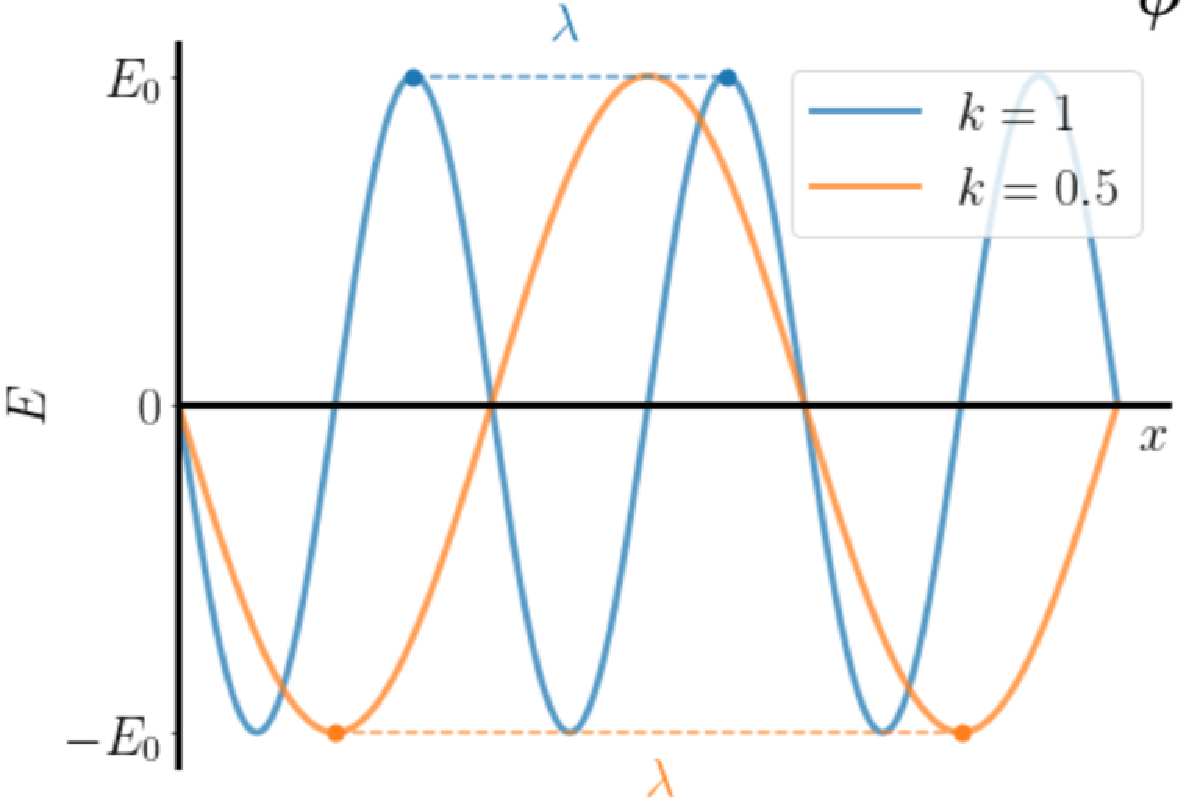
\includegraphics[width=0.8\textwidth]{lesson6/k.pdf}
        \caption{Two independent waves with $k=1, k=0.5$}    
    \label{fig:two-waves}
\end{figure}

% phi = 0, phi = pi/2
\begin{figure}[H]
   \centering
    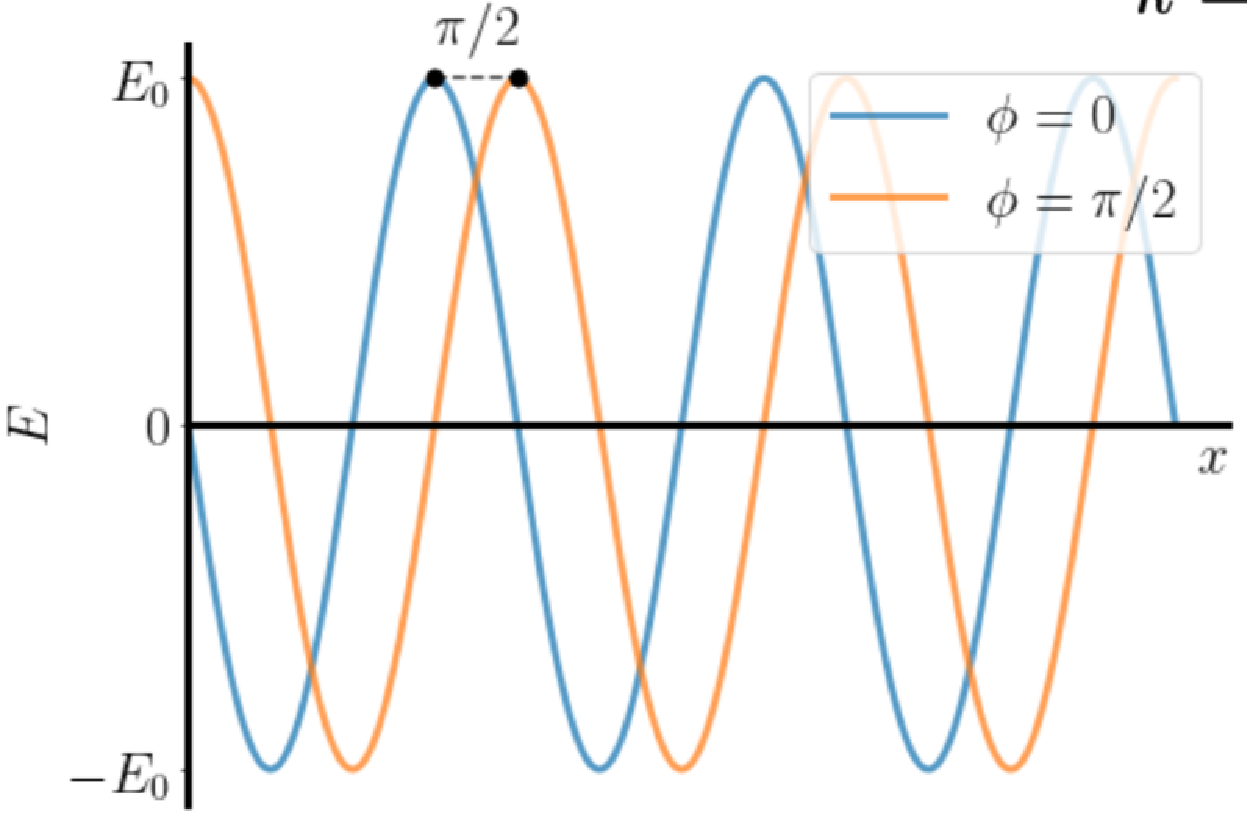
\includegraphics[width=0.8\textwidth]{lesson6/phi.pdf}
        \caption{Two waves with the same wavelength but different initial phase, $\phi = 0, \phi = \pi / 2$.}
    \label{fig:phase-diff-waves}
\end{figure}

% gif two waves [insert pic]
\begin{figure}[H]
   \centering
    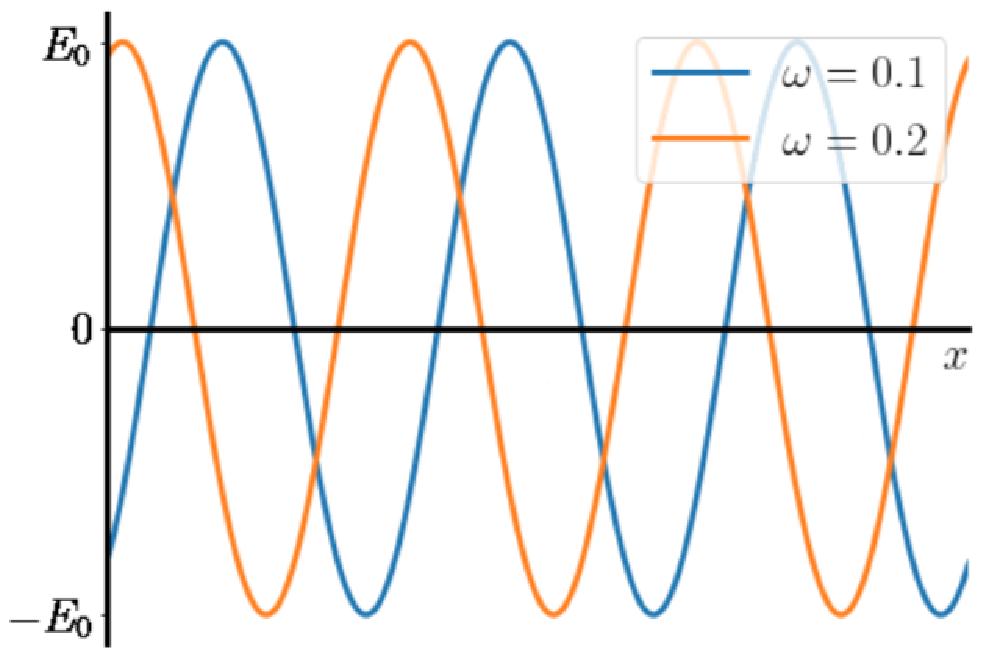
\includegraphics[width=0.8\textwidth]{lesson6/w.pdf}
        \caption{The same two waves as in the previous figure, after some time.  The orange wave propagates faster than the blue wave.}
    \label{fig:propagating-waves}    
\end{figure}

% superposition two waves
\begin{figure}[H]
   \centering
    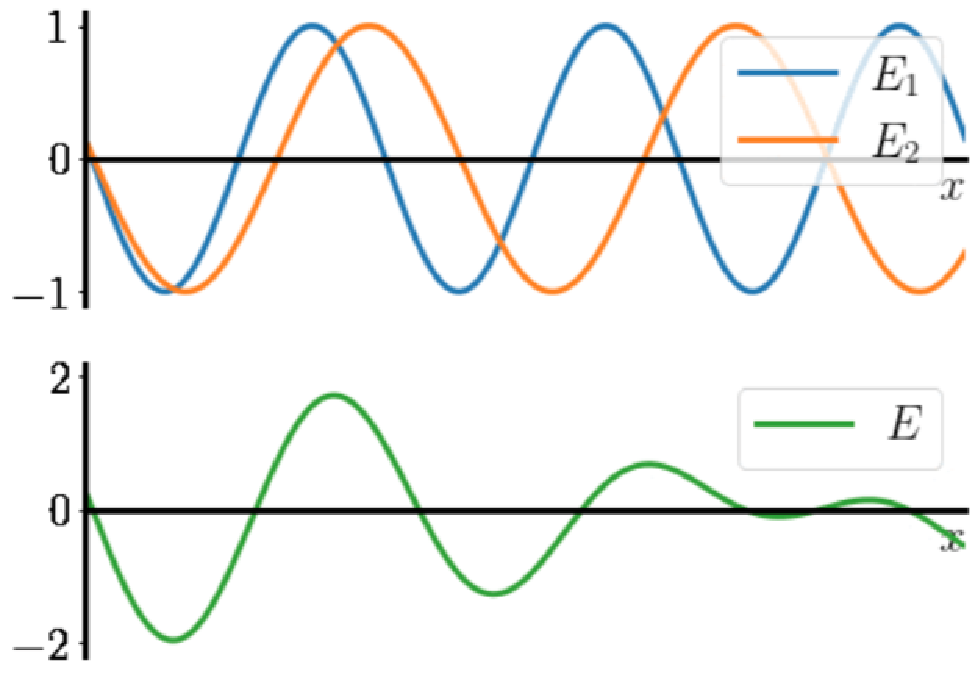
\includegraphics[width=0.8\textwidth]{lesson6/wave_superposition.pdf}    
        \caption{Waves in superposition. Notice the decay of the green wave as the two component waves move from in phase to out of phase.}
    \label{fig:decaying-superposition}    
\end{figure}

%%%%%%%%%%%%%%%%%%%%%%%%%%%%%%%%%%%%%%%%%%%%%%%%%%%%%%%%%%%%%%%%%%%%%%%%%%%%%%%%
\section{Phase and group velocities}
%%%%%%%%%%%%%%%%%%%%%%%%%%%%%%%%%%%%%%%%%%%%%%%%%%%%%%%%%%%%%%%%%%%%%%%%%%%%%%%%

\begin{equation}
E=E_{0} \sin (\omega t-k x-\phi)
\end{equation}


$\theta=\omega t-k x-\phi$

\begin{equation}
E=\sin (0.1 t-x)
\end{equation}

% graph, black dot
\begin{figure}[H]
   \centering
    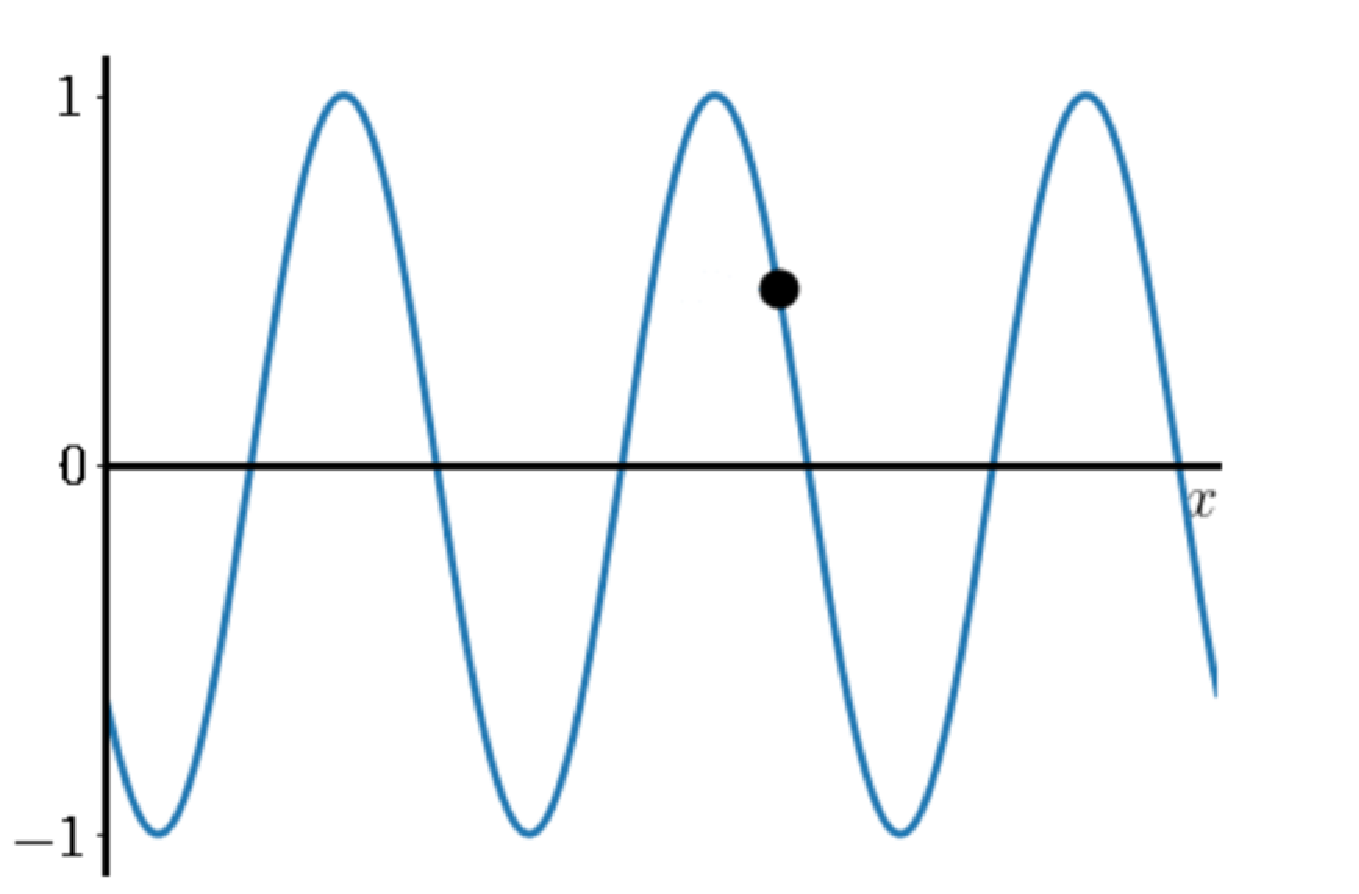
\includegraphics[width=0.8\textwidth]{lesson6/black_dot.pdf}
    \label{fig: 1}
    
        \caption{Phase velocity of a single wave.}
    
\end{figure}

\begin{equation}
\begin{aligned}
&E_{1}=E_{0} \sin \left(\omega_{1} t-k_{1} x\right) \\
&E_{2}=E_{0} \sin \left(\omega_{2} t-k_{2} x\right)
\end{aligned}
\end{equation}

\begin{equation}
\begin{aligned}
E &=E_{1}+E_{2} \\
&=E_{0}\left[\sin \left(\omega_{1} t-k_{1} x\right)+\sin \left(\omega_{2} t-k_{2} x\right)\right] \\
&=2 E_{0} \sin \left[\frac{\omega_{1}+\omega_{2}}{2} t-\frac{k_{1}+k_{2}}{2} x\right] \\
& \times \cos \left[\frac{\omega_{1}-\omega_{2}}{2} t-\frac{k_{1}-k_{2}}{2} x\right]
\end{aligned}
\end{equation}

\begin{equation}
E=2 E_{0} \sin \left[\frac{\omega_{1}+\omega_{2}}{2} t-\frac{k_{1}+k_{2}}{2} x\right] \times \cos \left[\frac{\omega_{1}-\omega_{2}}{2} t-\frac{k_{1}-k_{2}}{2} x\right]
\end{equation}

\begin{equation}
v_p = \frac{\omega_{1}+\omega_{2}}{k_{1}+k_{2}}
\end{equation}

\begin{equation}
v_g = \frac{\omega_{1}-\omega_{2}}{k_{1}-k_{2}}
\end{equation}

\begin{equation}
\begin{aligned}
&E_{1}=\sin (0.1 t-2.0 x) \\
&E_{2}=\sin (0.2 t-2.1 x)
\end{aligned}
\end{equation}

% t = 0 graph
\begin{figure}[H]
   \centering
    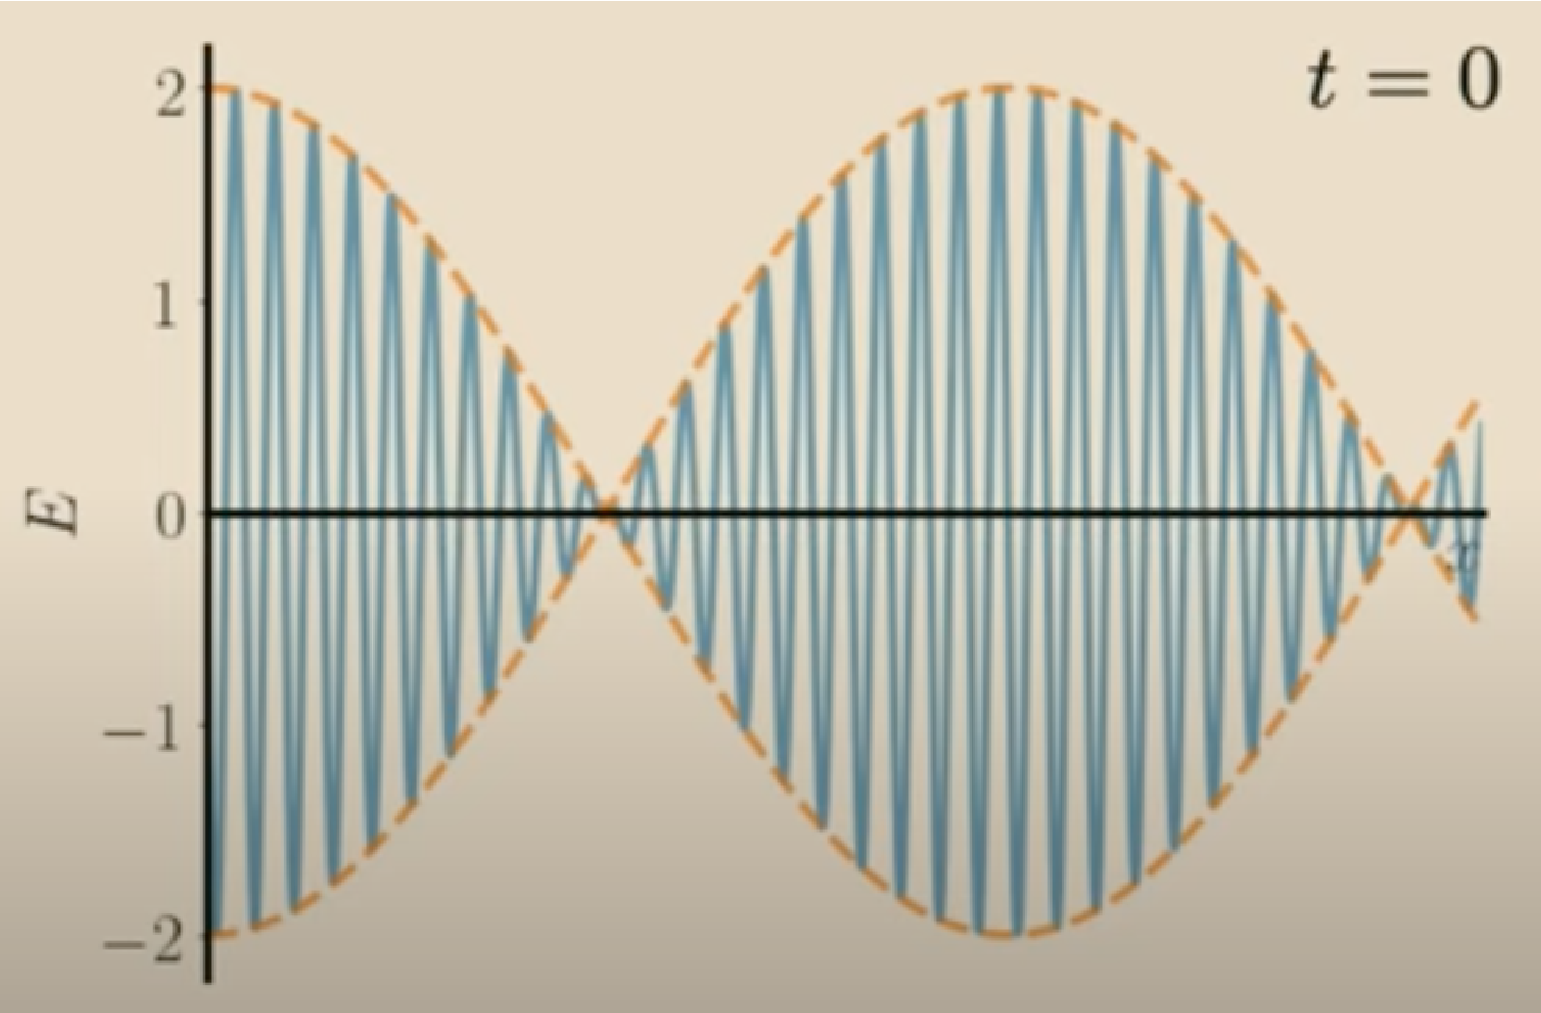
\includegraphics[width=0.8\textwidth]{lesson6/t=0.pdf}
    \label{fig: 1}
    
        \caption{}
    
\end{figure}

\begin{equation}
\begin{gathered}
v_{p}=\frac{\omega_{1}+\omega_{2}}{k_{1}+k_{2}}=\frac{0.3}{4.1} \approx 0.07 \\
%v_{g}=\frac{\omega_{1}-\omega_{2}}{k_{1}-k_{2}}=1 & 
v_{g}=\frac{\omega_{1}-\omega_{2}}{k_{1}-k_{2}}=1 
\begin{array}{l}
\end{array} \\
v_{g}>v_{p} \quad v_{g} \approx 14 v_{p}
\end{gathered}
\end{equation}

% red square, black dot
\begin{figure}[H]
   \centering
    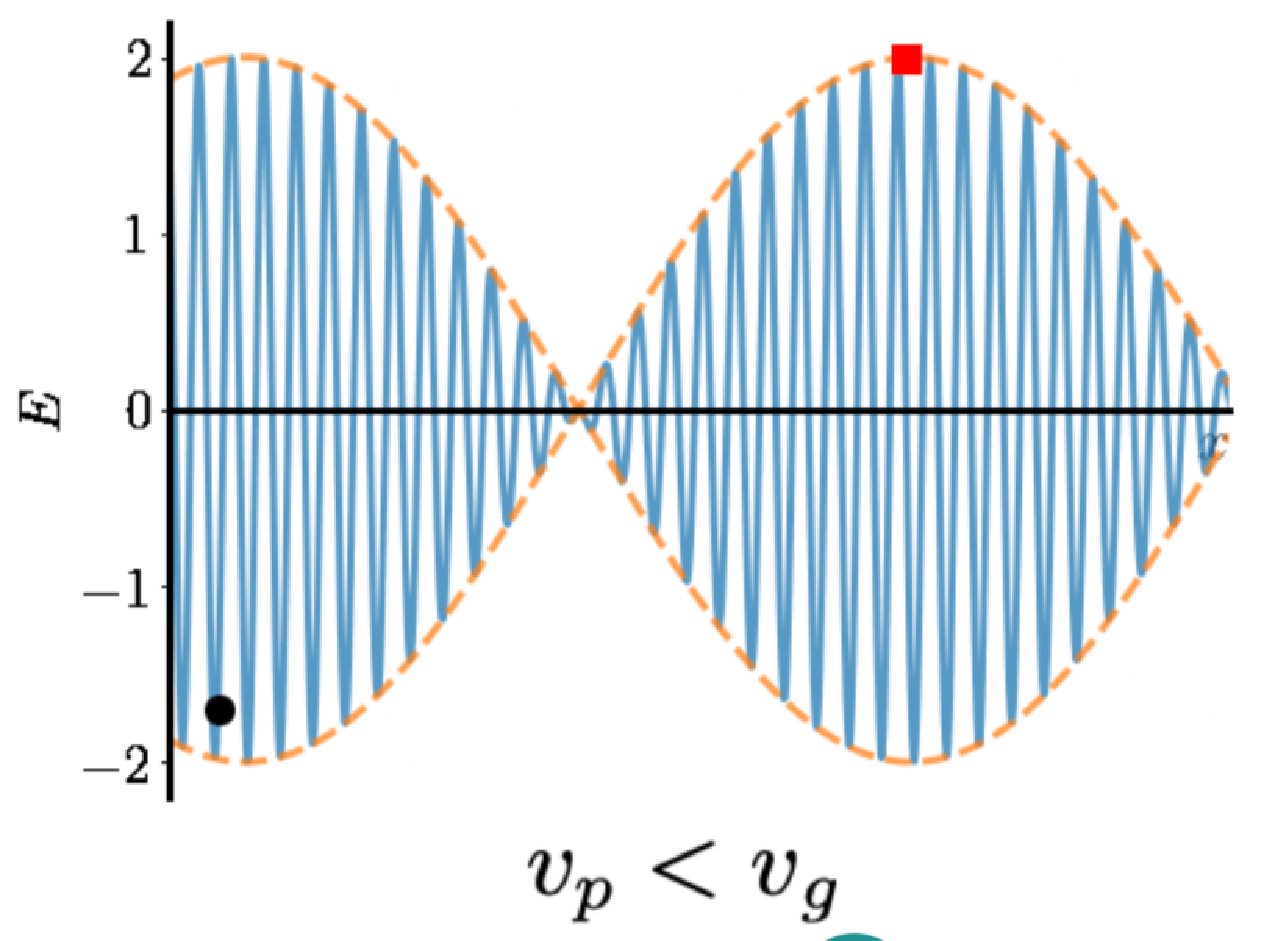
\includegraphics[width=0.8\textwidth]{lesson6/vp_less_vg.pdf}
    \label{fig: 1}
    
        \caption{A superposition with $v_p < v_g$.}
    
\end{figure}

\begin{equation}
\begin{aligned}
&E_{1}=\sin (0.1 t-0.1 x) \\
&E_{2}=\sin (0.2 t-0.2 x)
\end{aligned}
\end{equation}

% vp = vg
\begin{figure}[H]
   \centering
    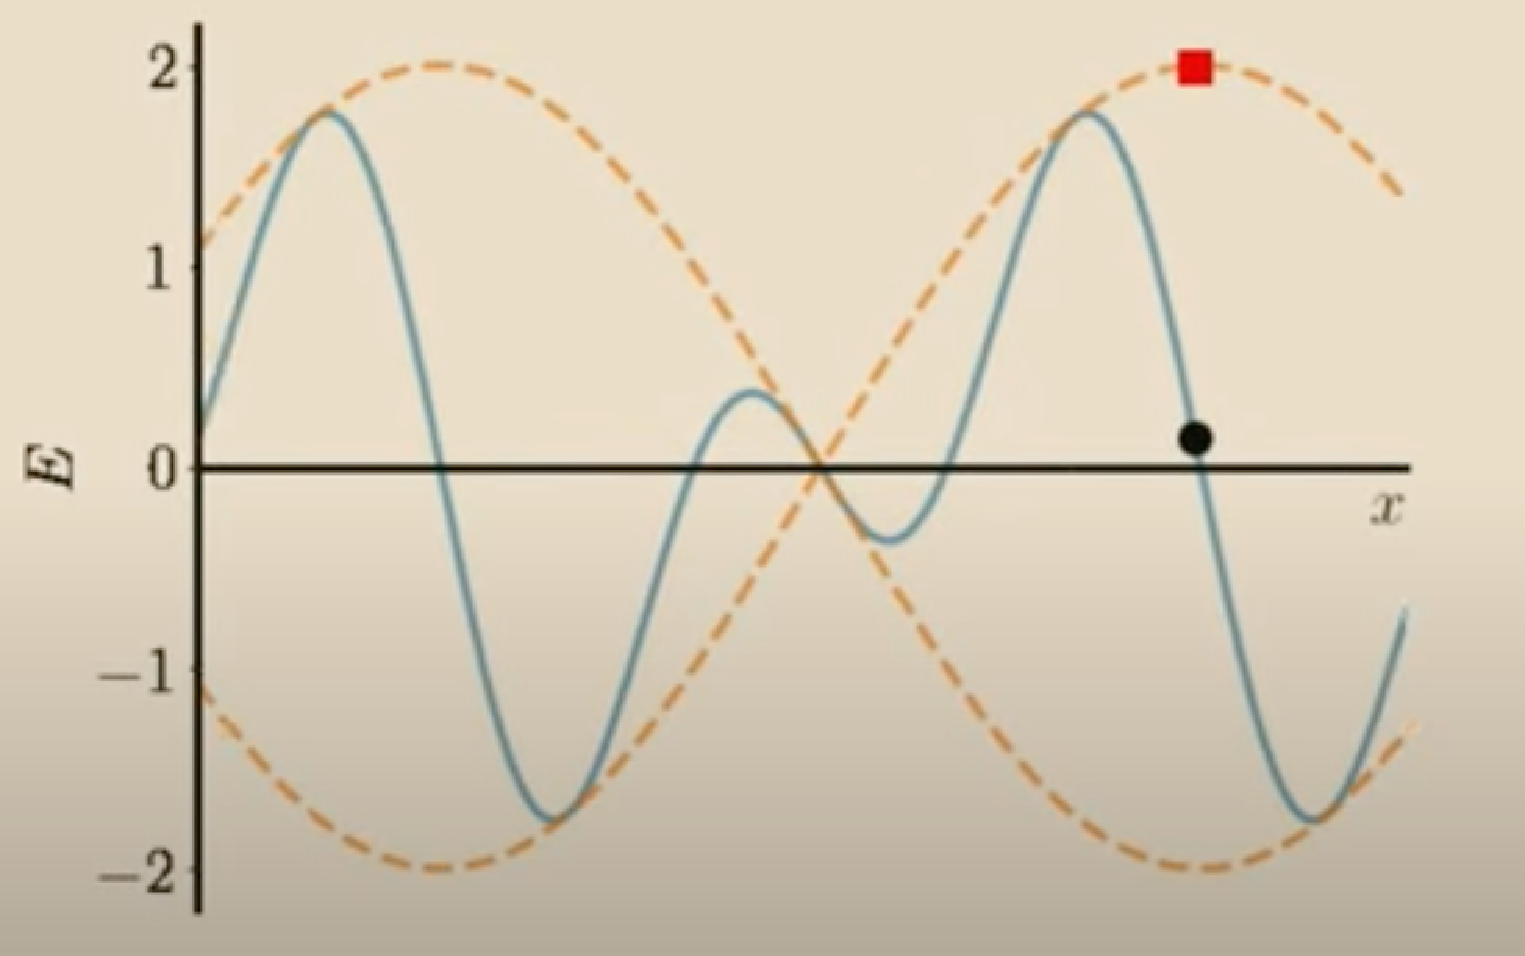
\includegraphics[width=0.8\textwidth]{lesson6/vp_equal_vg.pdf}
    \label{fig: 1}
    
        \caption{A superposition with $v_p = v_g$}
    
\end{figure}

\begin{equation}
\begin{aligned}
&E_{1}=\sin (0.1 t-2.0 x) \\
&E_{2}=\sin (0.2 t-1.5 x)
\end{aligned}
\end{equation}
% vg < vp
\begin{figure}[H]
   \centering
    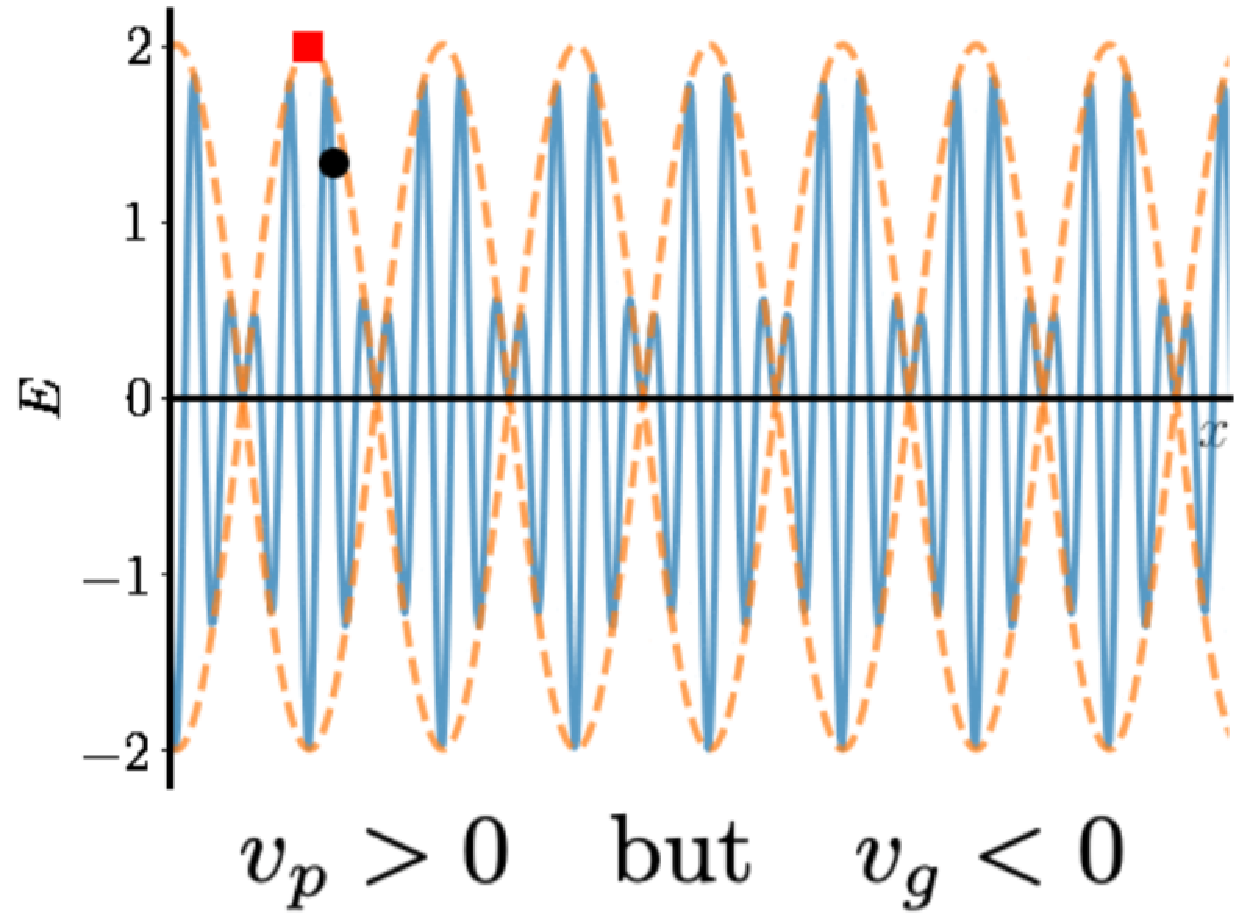
\includegraphics[width=0.8\textwidth]{lesson6/vp_greater_vg.pdf}
    \label{fig: 1}
    
        \caption{A superposition with $v_p > v_g$.}
    
\end{figure}

\begin{equation}
\begin{aligned}
E &=\sum_{k=2}^{3} \sin (-k x), \quad k \text { increasing in steps of } 0.1 \\
&=\sin (-2.0 x)+\sin (-2.1 x)+\ldots+\sin (-3.0 x)
\end{aligned}
\end{equation}

% pulse
\begin{figure}[H]
   \centering
    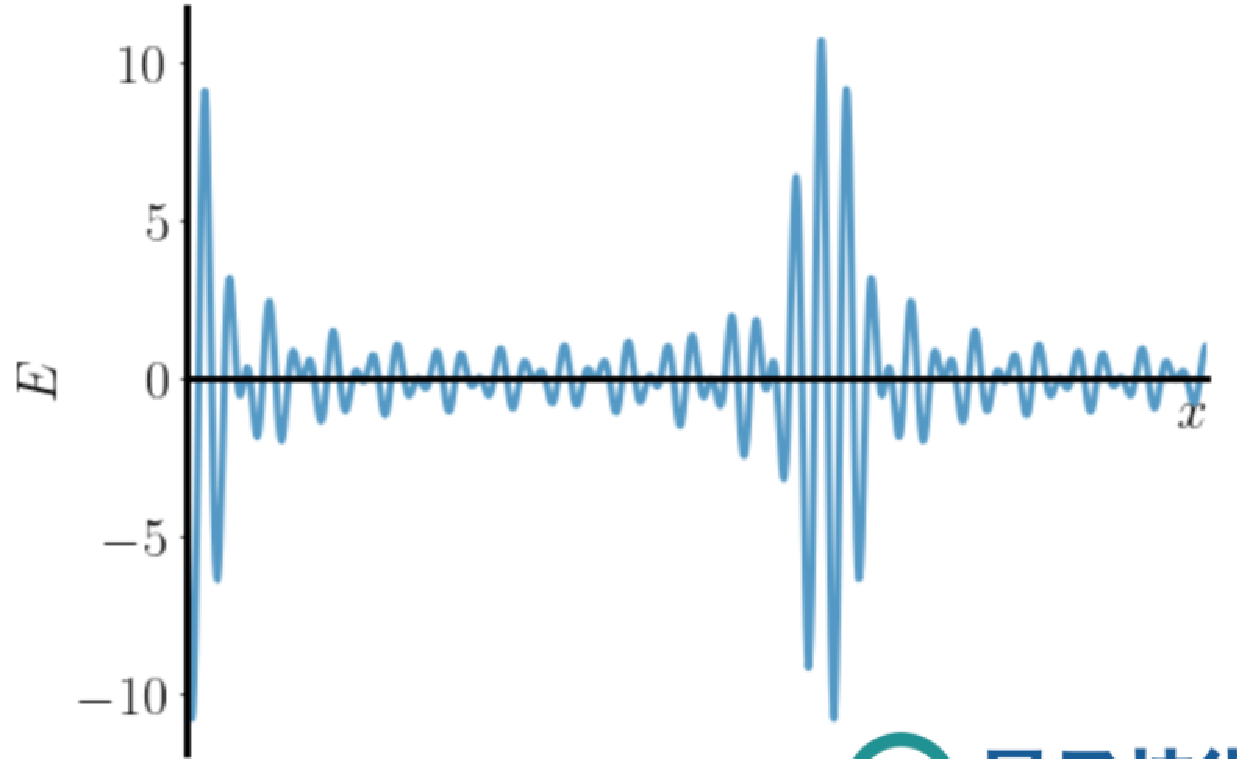
\includegraphics[width=0.8\textwidth]{lesson6/pulse.pdf}
    \label{fig: 1}
    
        \caption{}
    
\end{figure}

Step Two: Base and Group Velocities

In this step, we will get back to interference and see what effect it has on the speed with which waves propagate.

So first, let's consider a single wave of a single frequency propagating through space and ask the question: at what speed does this wave travel? We saw in the previous step that we can write down such a wave in this form- we've got the amplitude times sine of its phase. And maybe, you remember from previous studies that the wave velocity is given as the ratio of the wavelength lambda, and its period capital T. So we saw in the previous step that lambda is related to the wave number k as follows: lambda is equal to two pi over k. And similarly, the period of oscillation capital T is related to omega, the angular frequency, as two pi over omega. So substituting for lambda and substituting for T, we can obtain the expression for wave velocity in terms of omega and k as v, the wave velocity, is omega over k. So now we know how a single wave propagates. Let's consider when we have two waves that superpose together. Before we do that, let's look at an example. So we have a wave propagating at angular frequency zero point one and the wave number is one. And then, as you can see, I marked one black point here (follow pointer), this is a point of constant phase and it's propagating through space like that.

So now, what happens when we superpose two waves? At what velocity and what speed does the resultant superposition travel? Well, let's take two waves, and this time we allow their angular frequencies to be different, their wave numbers to be different, but for simplicity we consider these two waves to have same amplitude E naught.

When we add them together, we arrive at the following expression (see pointer): here both of them have some amplitude so we can just take out E naught out and write down the two waves in this form, and what we do next is we apply a trigonometric identity. That allows us to write this superposition E as a product of two wave signals. One is a sine signal and the other one is a cos signal. For the sine, the angular frequency is the following- (omega one plus omega two) over two, and the new wave number is (k1 plus k2) over two. And for the cos signal, we take the difference of the angular frequencies omega one and omega two, and the wave numbers k1 and k2. So let's have a look at the shape of this superposition. We said that we've got these two terms (sine and cos) that determine our superposition. If we only look at the sine, we see that it's oscillating at a much faster frequency, because here we are adding the angular velocities omega one and omega two, and we are adding the wave numbers k1 and k2. Whereas the other term, the cosine term, we call that the slow oscillating term because the new angular frequency is dependent on the difference between omega one and omega two, and the difference between k1 and k2. So, we define the phase velocity as the velocity of this fast oscillating term. So previously, we said that for a single wave it's just omega over k, but here, we saw that this omega ones and omega twos result in this new angular frequency for the fast oscillations, and this new wave number for the fast oscillations, so v-p, the phase velocity, is equal to omega one plus omega two divided by k1 plus k2.

And the group velocity is defined in a similar way but for the slow oscillations. So v-g, which we denote group velocity, is omega one minus omega two divided by k1 minus k2. So from this you can immediately see that even though we have a single wave, single superposition, there are these two notions of a phase velocity and group velocity which are not necessarily the same, they can be different, and we will see that later in this step.

So let's illustrate it with an example. We consider two waves E1 an E2. They have different angular frequencies, E1 has angular frequency zero point one, whereas E2 has angular frequency zero point two, and they have different wave numbers, E1 has two point zero, and E2 has two point one. So, let's plot this initially at time equals to zero, and as we said, we expect the shape of the superposition to to be composed of two waves. One is this fast oscillating blue line, and on top of that we have this slowly varying envelope. Again, this blue fast oscillating term is given by the sine term from previous slides, and this orange dashed line gives us the envelope which is proportional to the cosine. Now let's get things moving, and in time again it propagates through space.

So now, let's actually compute what the phase and group velocities are for our example. We just substitute into our expressions for phase velocity, so omega one plus omega two, we just add them together, so 0.1 plus 0.2 is 0.3. k1 plus k2, again we add them together, 2.0 plus 2.1 is 4.1. And this (v-p) is approximately 0.07 (zero point zero seven). For the group velocity, we do the same thing and we obtain that the group velocity is equal to one. So we can see that the group velocity in this case is larger than the phase velocity, and in fact it's about fourteen times larger. So let's get back to our propagating wave, and here you can see what actually happens to the points on our wave. So this black dot oscillating up and down represents our phase velocity. This black point is moving through space with the phase velocity, so you can see that it's moving up and down quite a lot, but actually it's not propagating through space very much, because it's in this example equal to 0.07, whereas this red square that occasionally you can see at the top, that goes zooming- it's sitting on the envelope over there and it goes to zooming through space. That point represents the group velocity. Well you can't actually see that it's fourteen times faster but mathematically that's true. And as we said in this case that we picked the phase velocity is smaller than the group velocity. But this is not always the case.

Let's look at this following example: we kept the same angular frequencies for the two waves, but we changed the wave numbers. Now E1 has k equal to zero point one and E2 has k equal to zero point two. Let's see what that looks like. As you can see, now the group velocity and the phase velocity are the same. The black point and the red square move at the same velocity.

So far, we have looked at cases when both velocities are in the same direction. Now, let's look at a very peculiar case.

Again, we keep the angular frequencies fixed, but this time we change k1 to two point zero and k2 to one point five, and let's see what happens. You see that again, the black dot representing our phase velocity is moving in the positive x direction as was the case before, but on the other hand this red square is moving backwards, because the group velocity in this case is actually negative. So you can see that you can have a lot of fun with the group and phase velocities. there are many different scenarios depending on omega one and omega two and k1 and k2.

And so far, we have been looking at superposition of only two waves. What happens if we consider superposition of more than two waves?

Let's consider a particular example where our superposition is given as a sum of some very simple waves. Here, we have frozen time and basically set t equals to zero, so we only have sine of minus kx, where this k vary from two to three in steps of zero point one. So really, what we have is a sum of sine of minus 2x, plus a sine of minus 2.1x, and so on until we reach the 11th term of sine minus 3x. And in fact, what we get is the following shape: what we call this shape is a "pulse". You can see that for most of x, the superposition is close to zero. There are some disturbances, there are some oscillations, but they're close to zero, and then suddenly constructive interference kicks in and you have this big pulse over there. And pulses are very important because using pulses, we can encode information so it's very important in communication theory.

\section{Interference with single photons}

% double_slit standard
\begin{figure}[H]
   \centering
    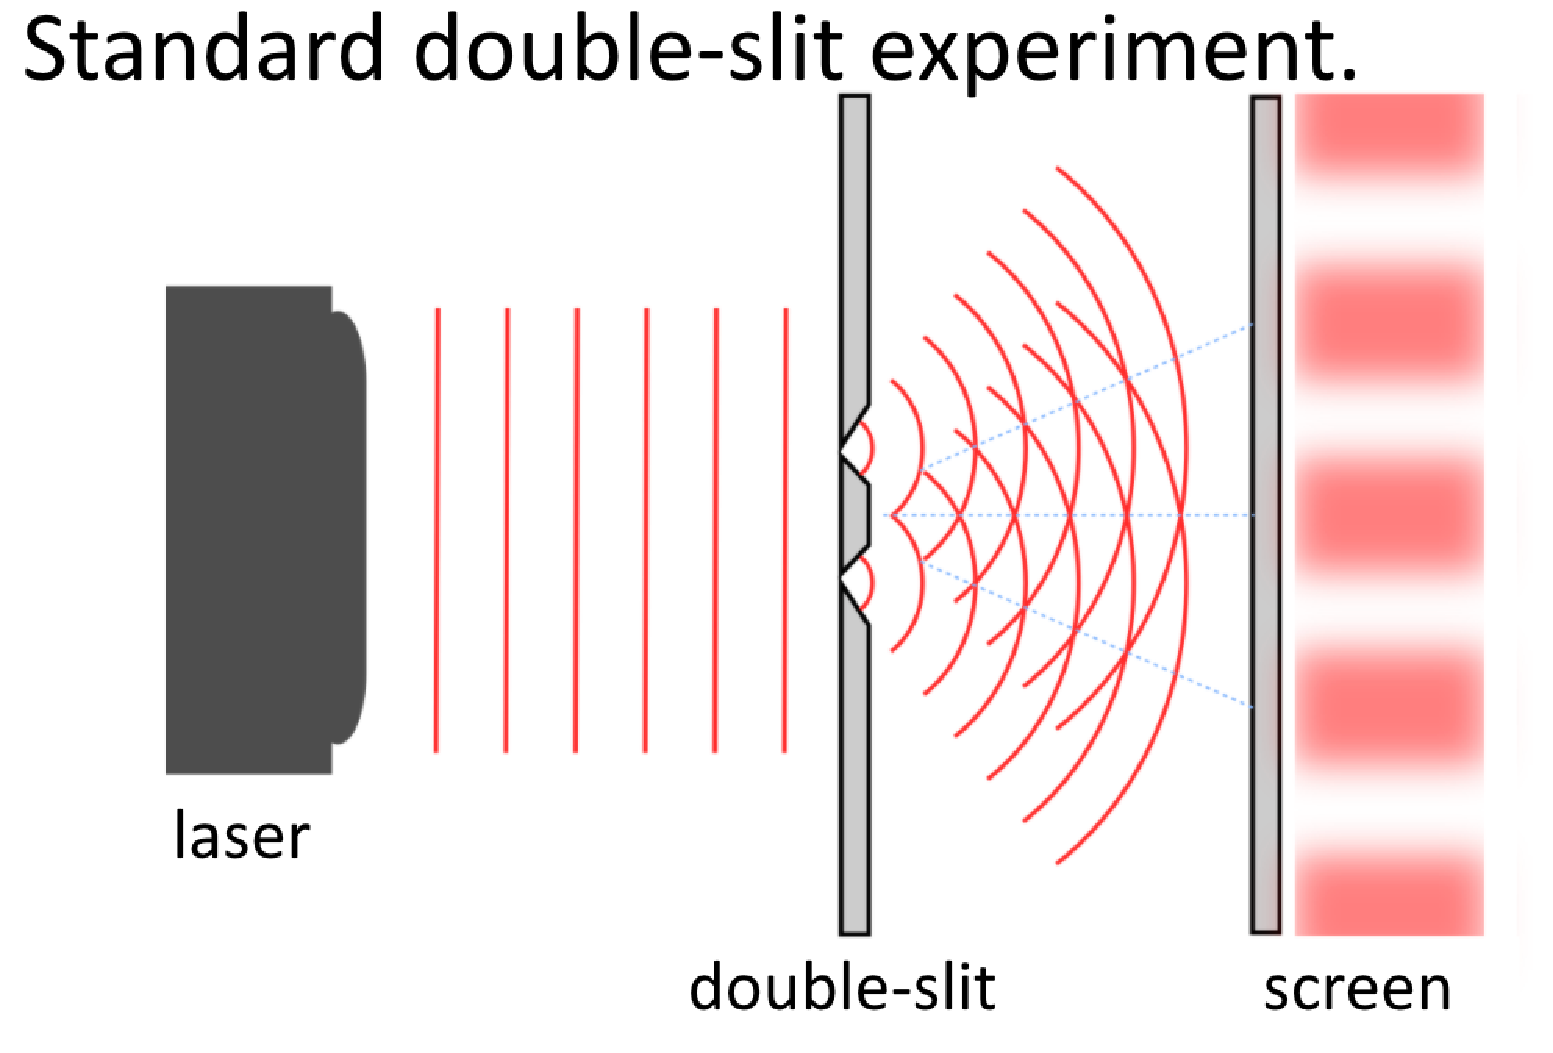
\includegraphics[width=0.8\textwidth]{lesson6/standard_double_slit.pdf}
    \label{fig: 1}
    
        \caption{The canonical two-slit experiment.}
    
\end{figure}

% constructive interference
\begin{figure}[H]
   \centering
    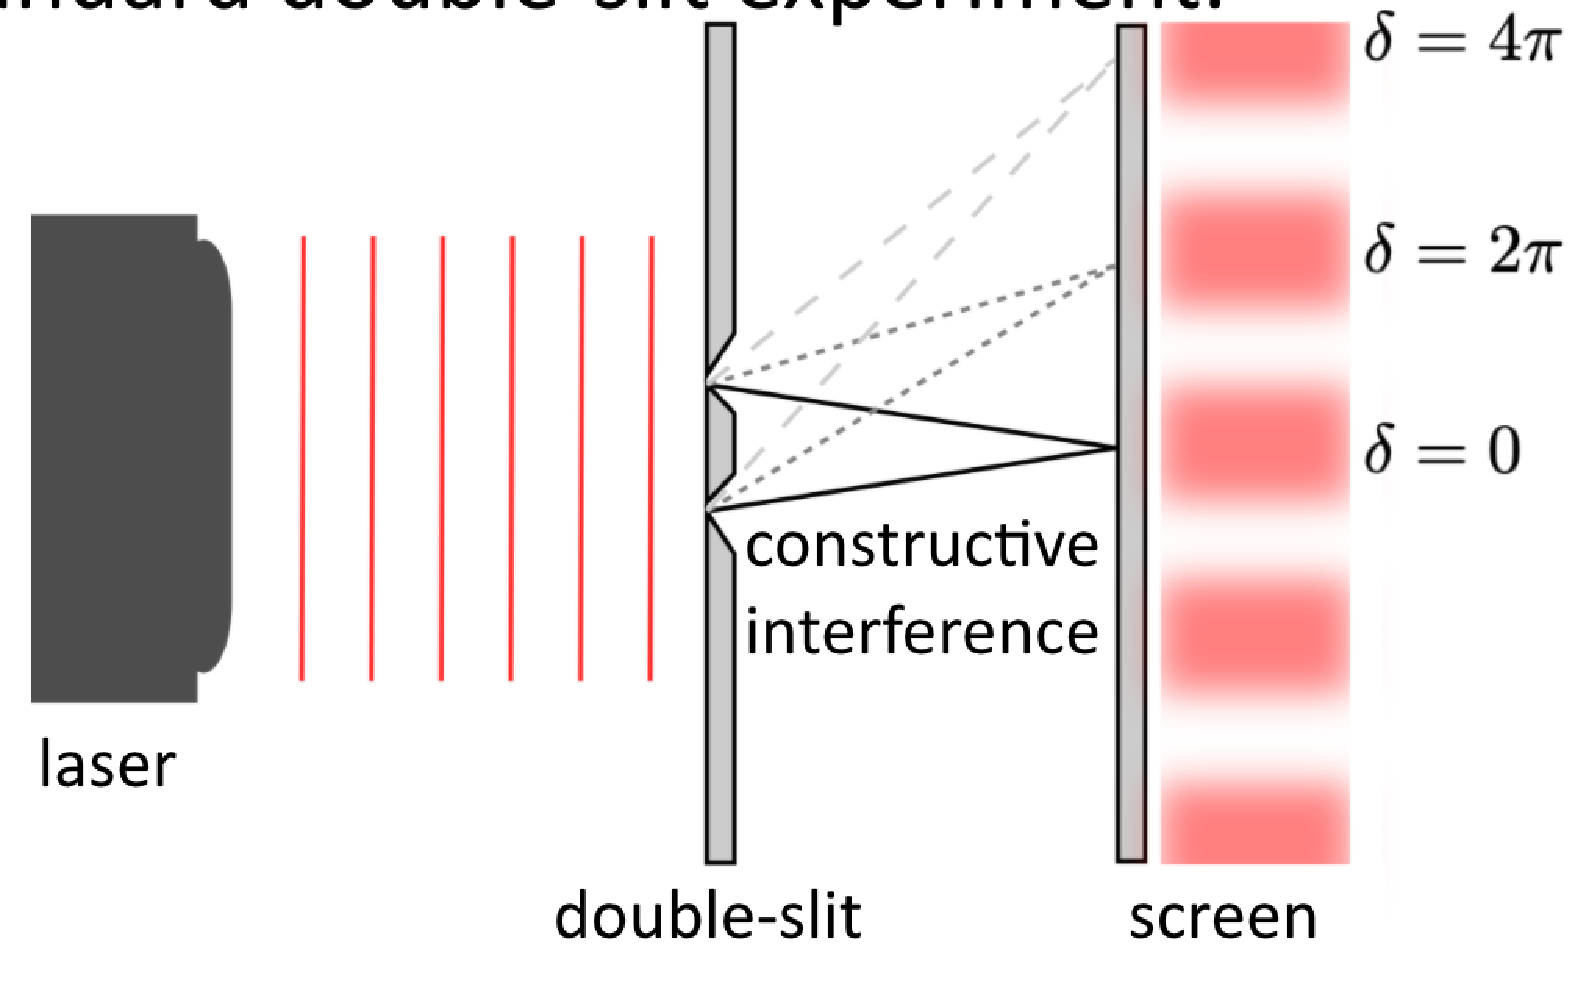
\includegraphics[width=0.8\textwidth]{lesson6/double_slit_constructive.pdf}
    \label{fig: 1}
    
        \caption{Constructive interference.}
    
\end{figure}

% destructive inteference
\begin{figure}[H]
   \centering
    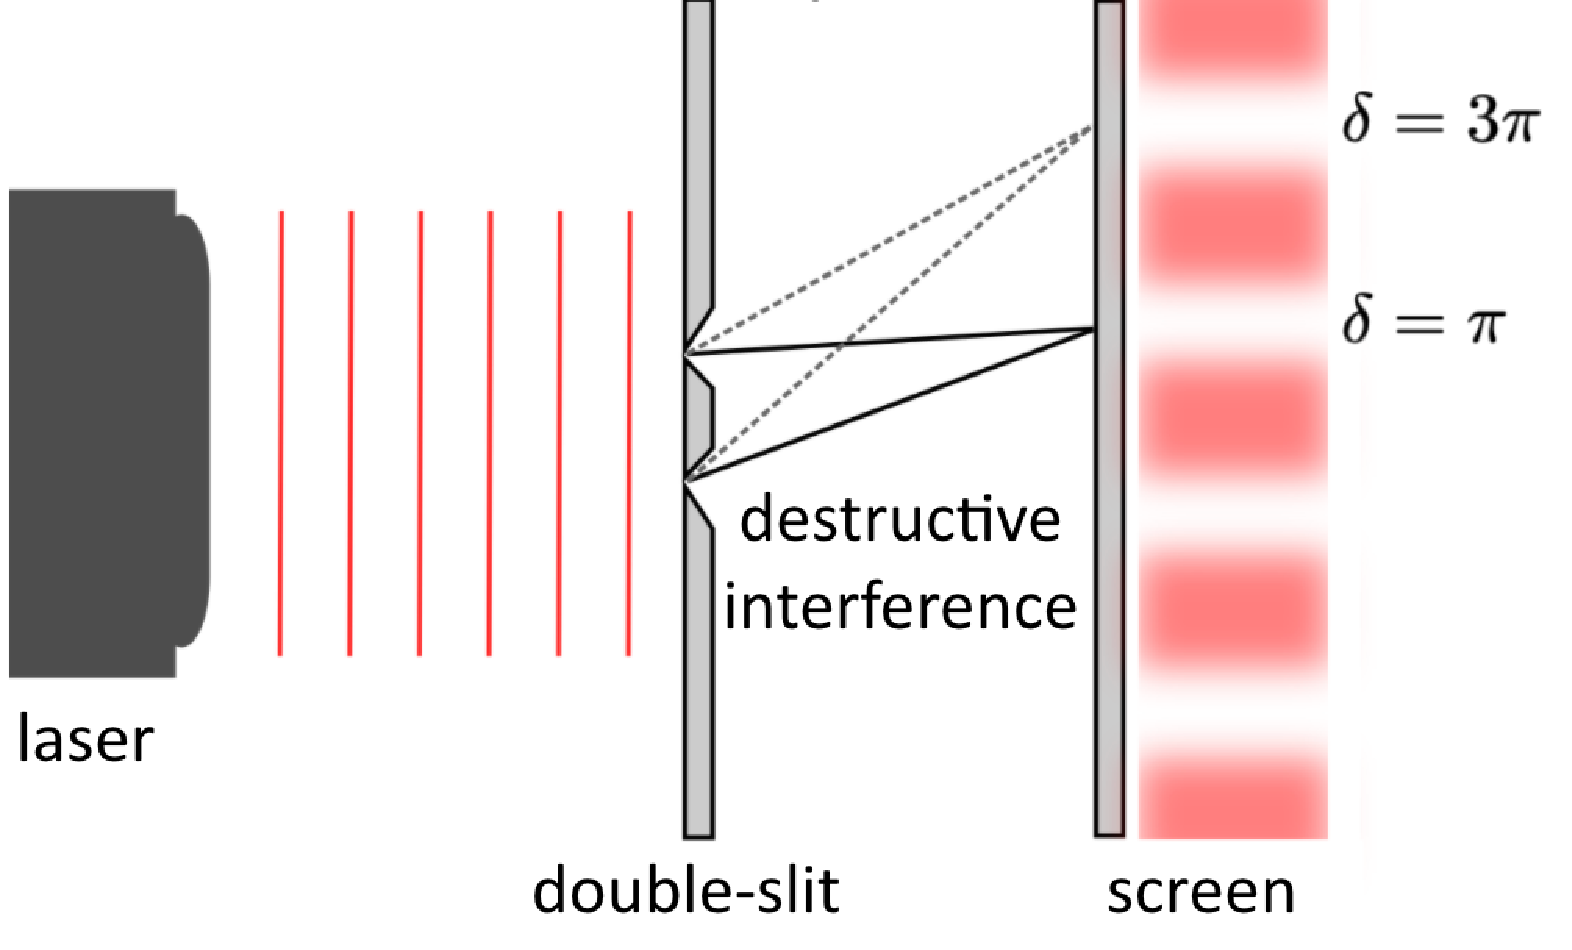
\includegraphics[width=0.8\textwidth]{lesson6/double_slit_destructive.pdf}
    \label{fig: 1}
    
        \caption{Destructive interference.}
    
\end{figure}

% attenuated laser
\begin{figure}[H]
   \centering
    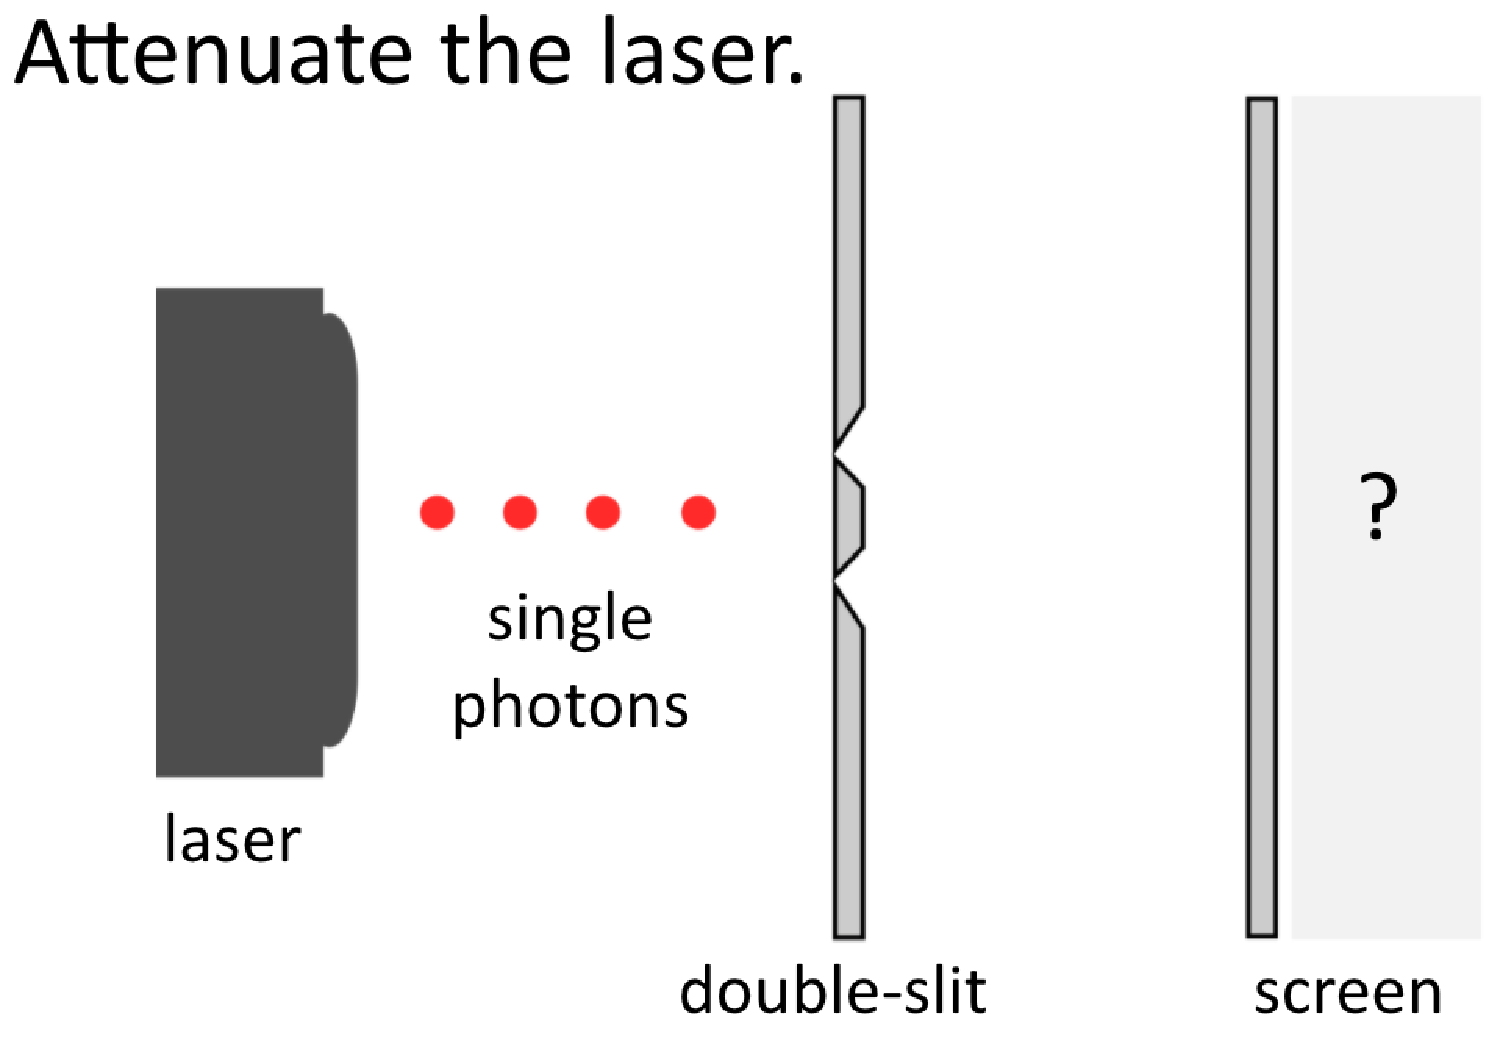
\includegraphics[width=0.8\textwidth]{lesson6/attenuate_laser.pdf}
    \label{fig: 1}
    
        \caption{Attenuated laser light.}
    
\end{figure}

% block bottom
\begin{figure}[H]
   \centering
    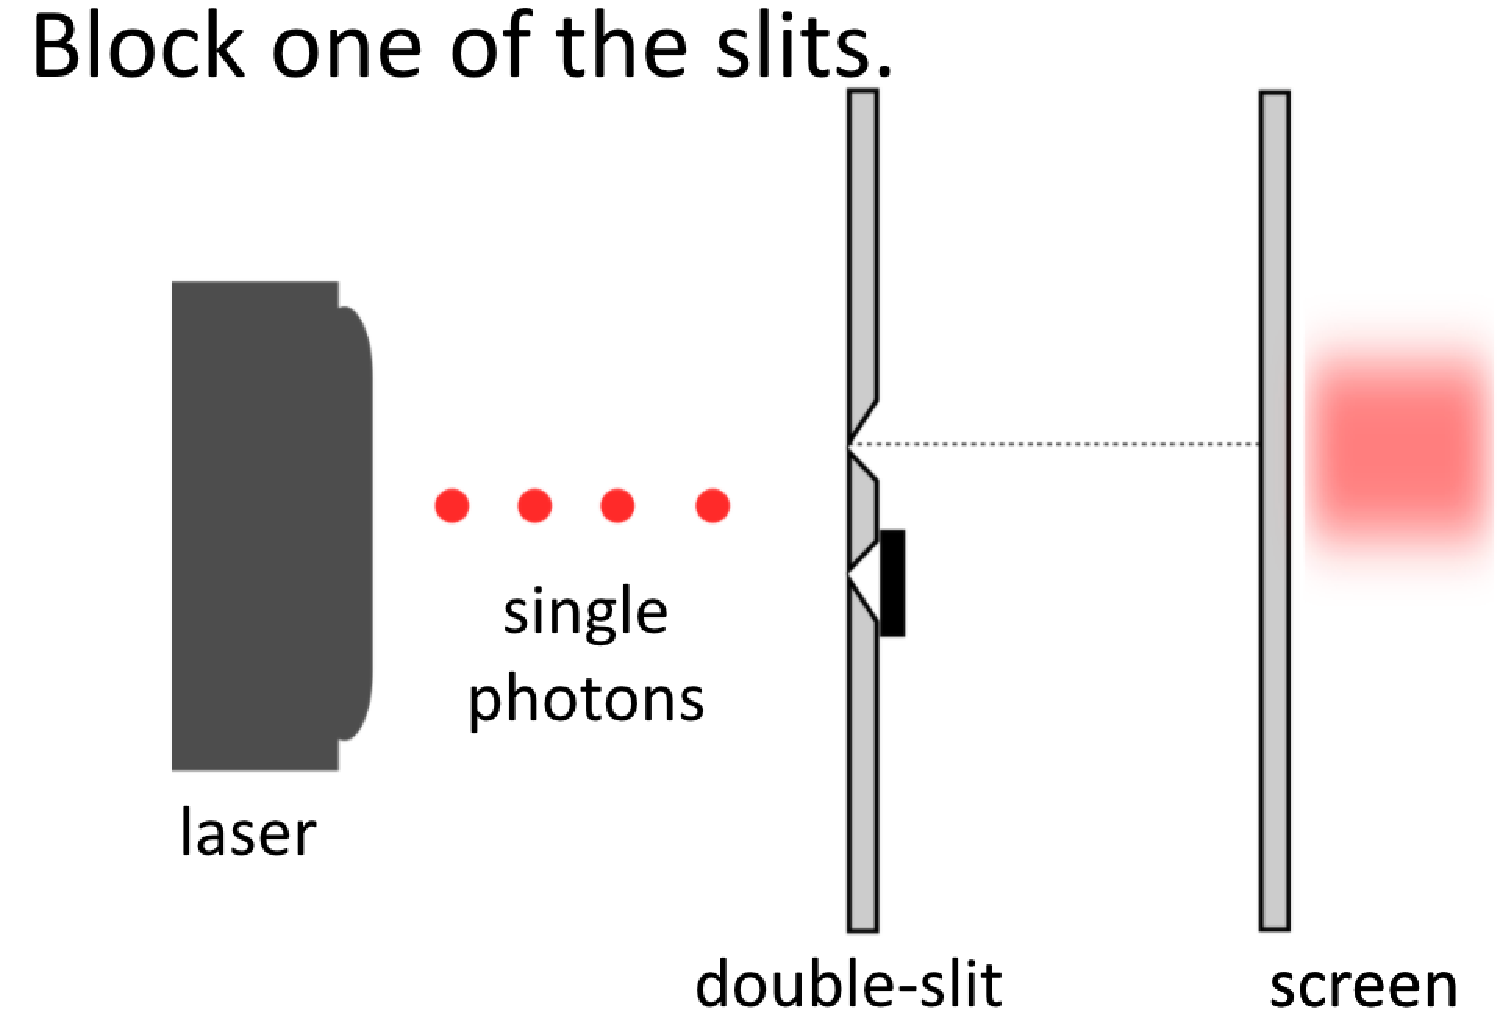
\includegraphics[width=0.8\textwidth]{lesson6/block_bottom.pdf}
    \label{fig: 1}
    
        \caption{Bottom of the block?}
    
\end{figure}

% block top
\begin{figure}[H]
   \centering
    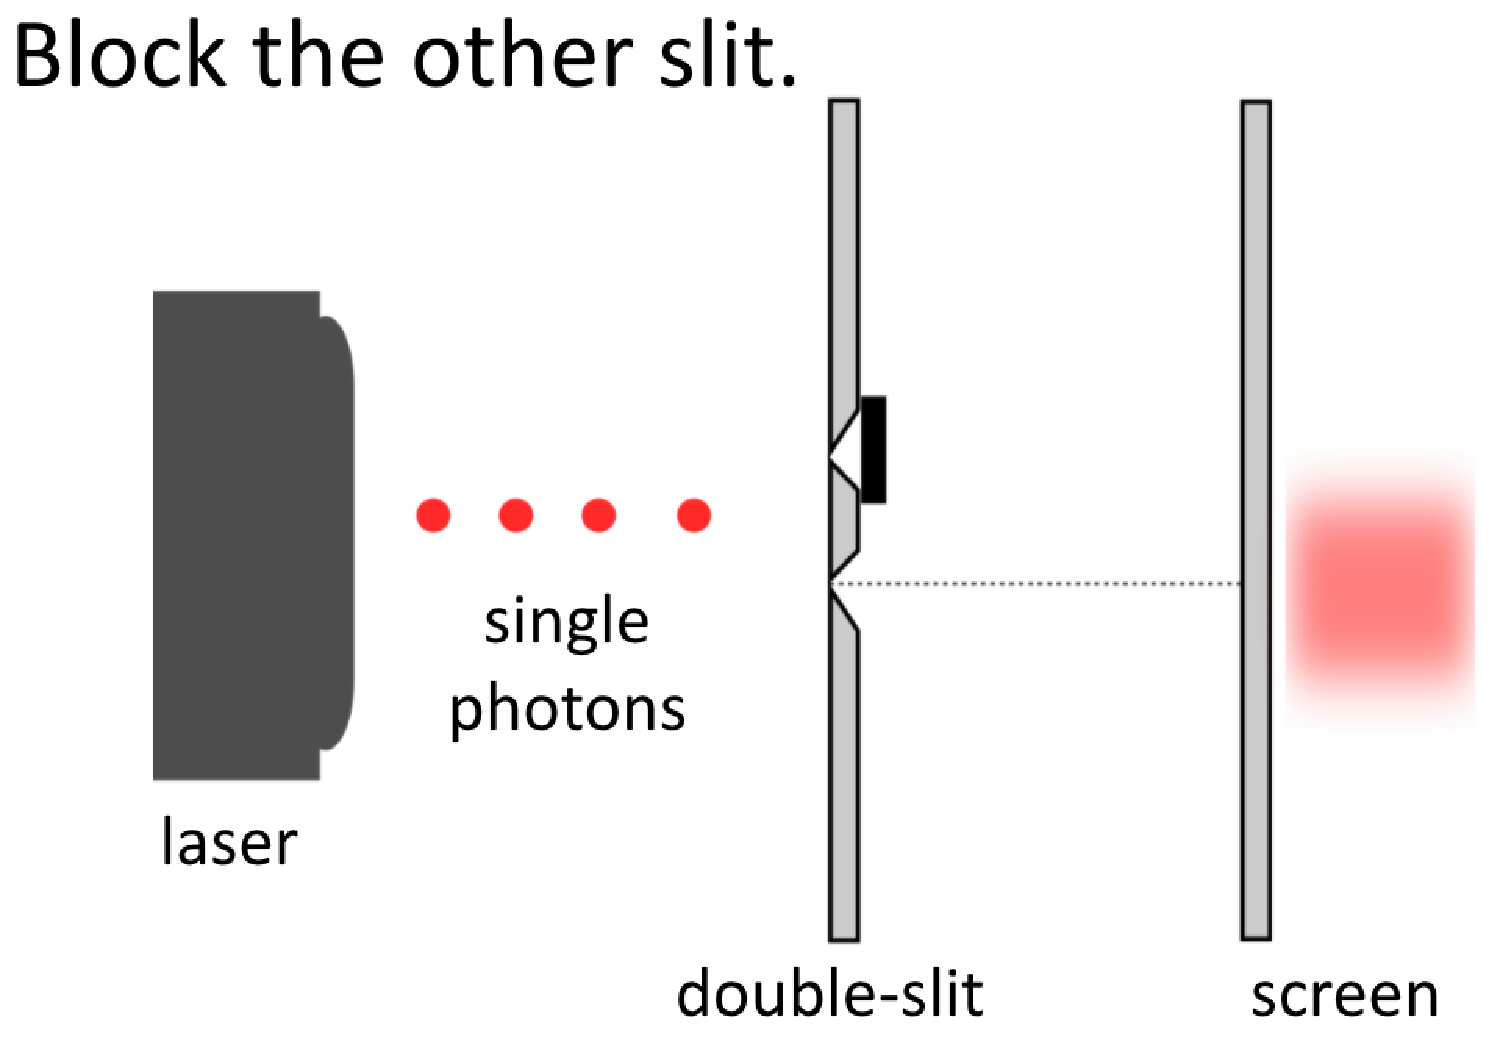
\includegraphics[width=0.8\textwidth]{lesson6/block_top.pdf}
    \label{fig: 1}
    
        \caption{Hole in the top of the block?}
    
\end{figure}

% block netiher expectation
\begin{figure}[H]
   \centering
    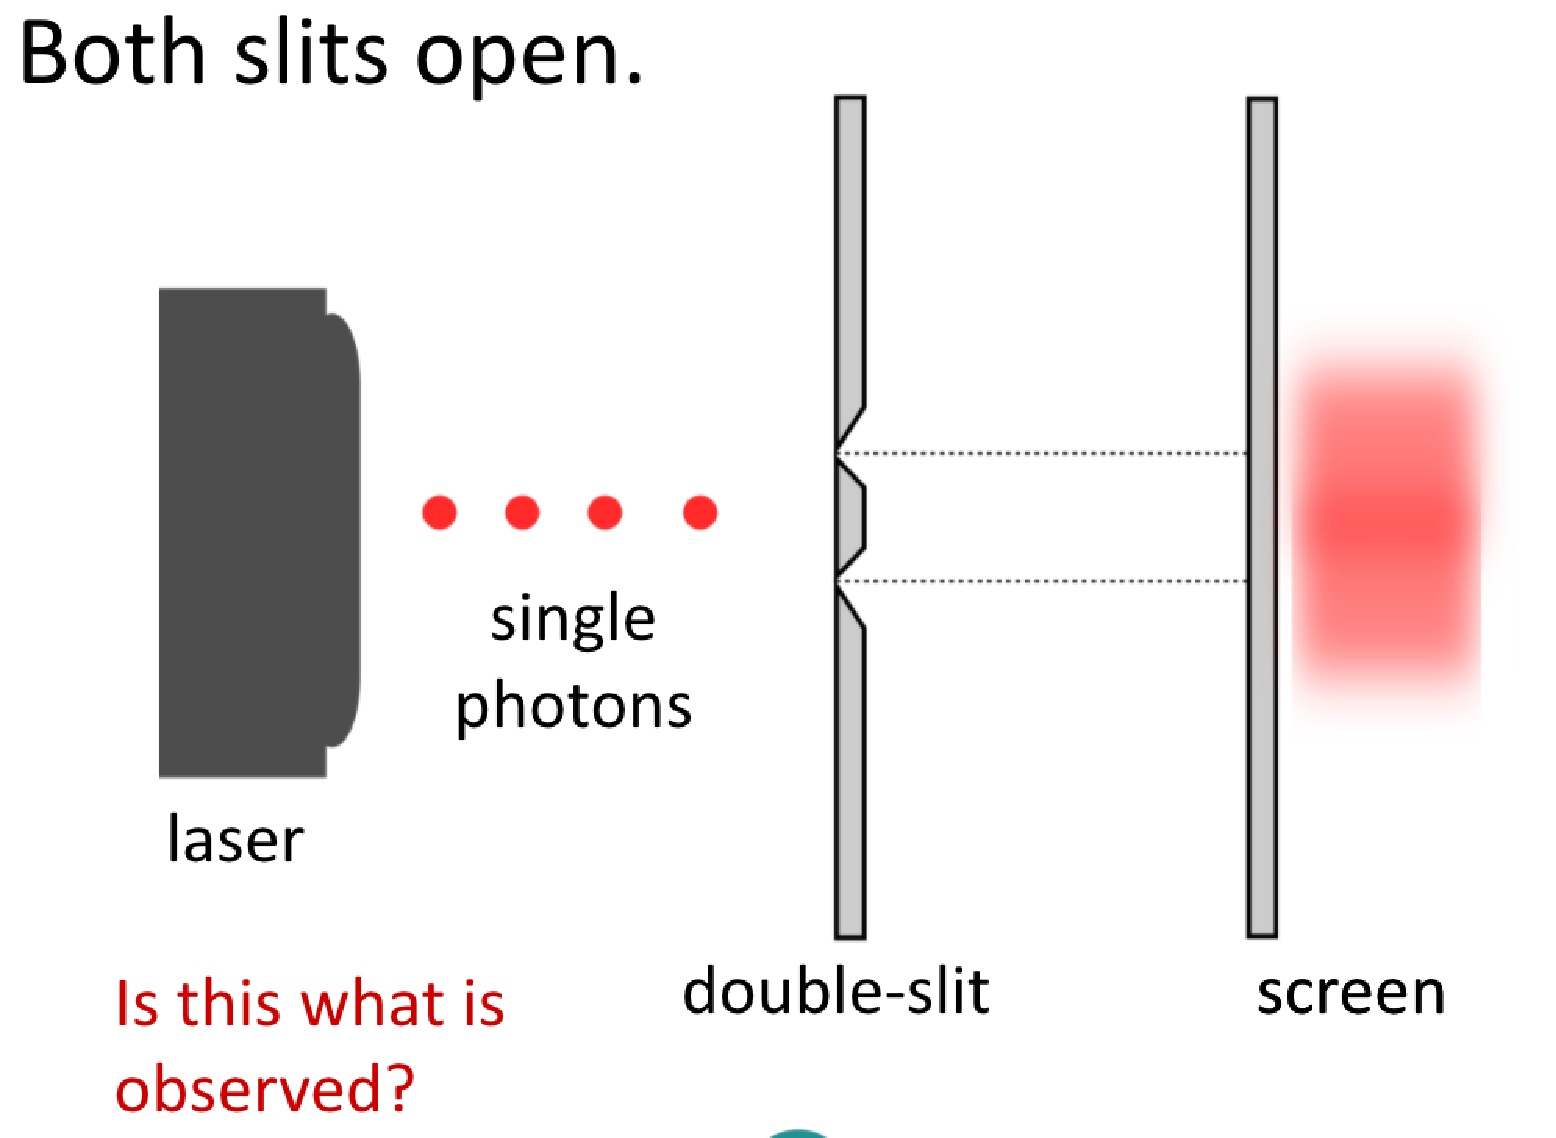
\includegraphics[width=0.8\textwidth]{lesson6/block_neither.pdf}
    \label{fig: 1}
    
        \caption{Neither: the idea?}
    
\end{figure}

% block neither reality
\begin{figure}[H]
   \centering
    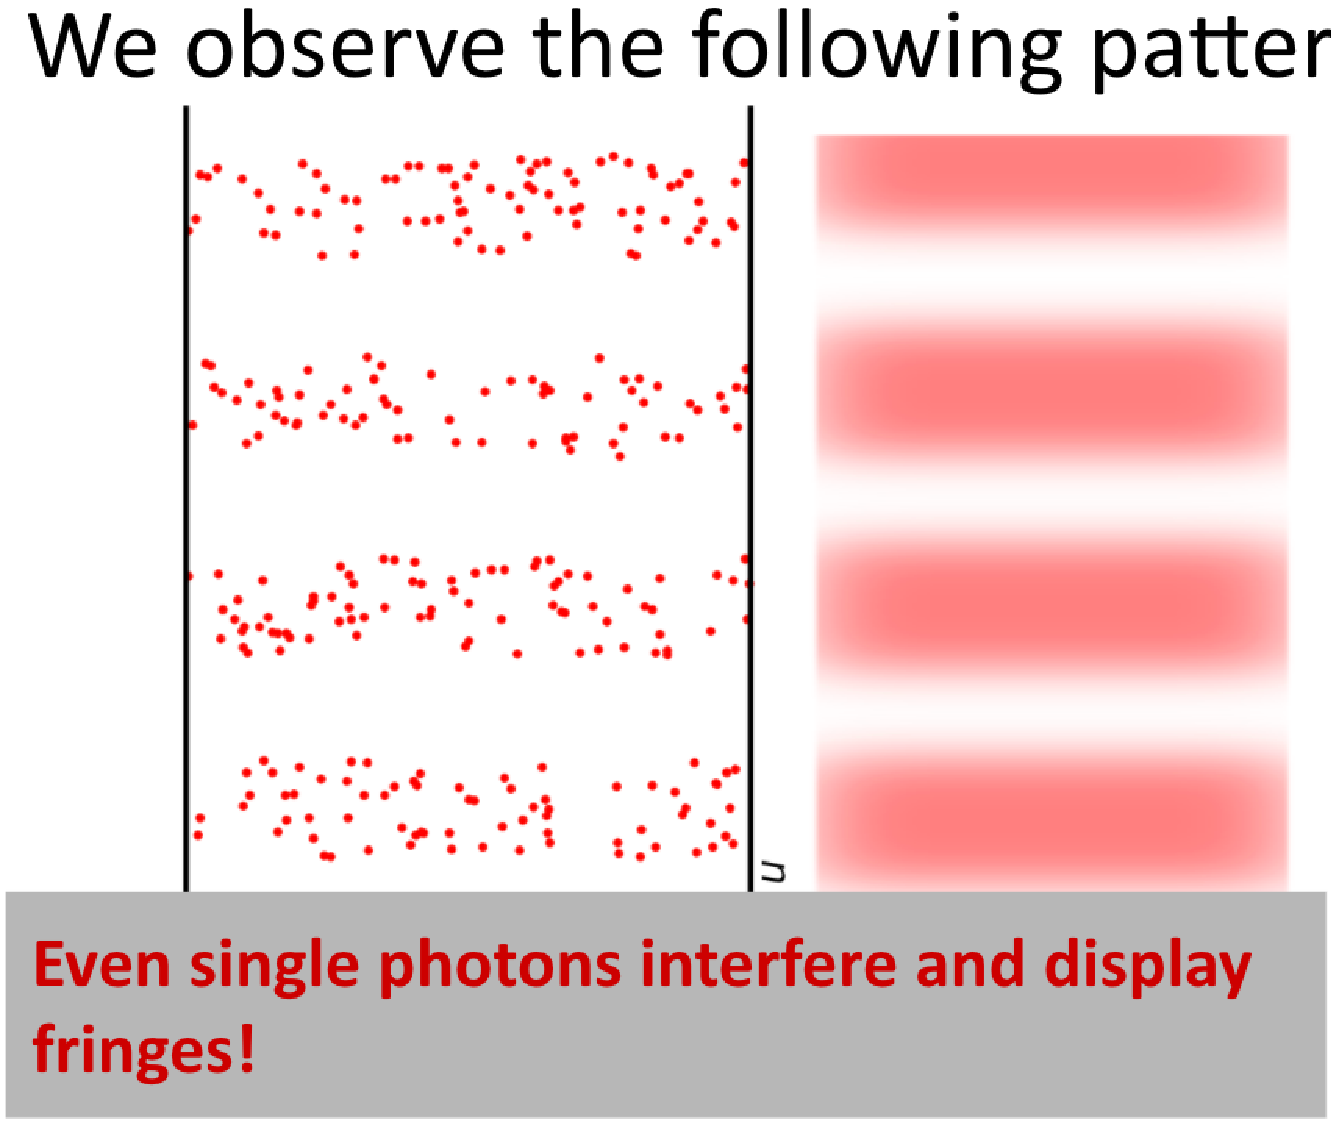
\includegraphics[width=0.8\textwidth]{lesson6/block_neither_reality.pdf}
    \label{fig: 1}
    
        \caption{Neither: the reality?}
    
\end{figure}

Step Three: Interference with Single Photons

I'm sure you have already seen the the scenario of a double slit experiment with laser light, but let's review it again.

In this experiment we've got a source of coherent light, so a laser. And it's turned on, and the laser light is incident on a screen, where there are only two small double slits where the light can go through, and then it propagates towards another screen where we detect a pattern. And the pattern that we see looks something like this: we've got fringes of bright light, and then these white fringes where there is no light. Why is that? As you can see, as the light is propagating through here (follow pointer), these lines, they represent the peaks of the electromagnetic wave, whereas the space in between them represent the valleys, the troughs. So as the two waves go through these slits, they have a chance to interfere constructively or destructively. Where their peaks meet, the wave- the interference of the two waves reinforces their amplitude. On the other hand, if a peak meets a trough or a valley, then the amplitudes cancel, and here we can see these light blue lines, these are the lines along which we see constructive interference.

For example, here we see the light coming from the top slit, light coming from the bottom slit, and they go towards the screen. The path length of these two paths are equal, therefore there is no phase difference between the two waves coming from the top slit and the bottom slit, and we observe constructive interference. On the other hand, for this other fringe, the path length for this top path is a little bit shorter than the bottom one. But the phase difference introduced for this case is exactly two pi, which again, corresponds to constructive interference as we have seen in the previous step. And similarly for the other fringes, for this top one, we have a phase difference of four pi.

On the other hand, if we consider these other path (follow pointer), as we said, this is where peaks meet the troughs, so this is where the path differences are odd integer multiple of pi. So for this first dark region on the screen, we've got the the phase difference being pi, for the second dark region on the screen we've got the phase difference being three pi.

Now, let's consider the scenario where we attenuate the laser light to such low levels that it's only firing single photons at a time, and furthermore, the level of attenuation is so high that we can be pretty sure that there's only one photon at a time between this screen where we place the double slits, and the screen where we are recording the pattern. So, what happens? Well, we know that the photons must go through one of these slits. So, let's try and cover one of them. What do we expect? If we cover the bottom one, then definitely the photons have to go through the top slit in order to hit the screen, so we expect most of the photons hitting the screen in this region that's the closest to the top slit. On the other hand, if we block the top slit and the photons are allowed to pass through this bottom slit, then we expect most of the photons to be recorded on the screen over here (see slide). What happens if we open both of the slits? Well. they can go through the top, and they can go through the bottom, so we expect something like this: we expect that the two previous distributions are just added together. Is this really what we see? Well, let's find out. In fact, what we see is the following: we start firing photos at the screen. Originally, there's not much pattern that we can discern, but as the time progresses, as more and more photons hit the screen, we can clearly see these fringes being formed. These fringes are the same fringes as we could see before with strong laser light as shown here. So let's just pause and appreciate really what's going on. We saw these fringes on the right with a strong laser light, and it wasn't very surprising, however here, somehow each individual photon knows that they still need to follow the same pattern, still they are drawn towards these bright fringes on the screen, and they avoid these dark fringes in between them. This is because of interference of different possible paths. Even though we always have a single photon in our interferometer, still it obeys the same rules of interference as if we had a strong laser pulse.


\section{Interference with qubits}

\begin{equation}
\begin{aligned}
|0\rangle &=\left(\begin{array}{l}
1 \\
0
\end{array}\right) \quad|1\rangle=\left(\begin{array}{l}
0 \\
1
\end{array}\right) \quad H=\frac{1}{\sqrt{2}}\left(\begin{array}{cc}
1 & 1 \\
1 & -1
\end{array}\right) \\
|0\rangle & \longrightarrow H|0\rangle=\frac{1}{\sqrt{2}}(|0\rangle+|1\rangle) \\
& \longrightarrow H\left[\frac{1}{\sqrt{2}}(|0\rangle+|1\rangle)\right] \\
&=\frac{1}{2}(|0\rangle+|1\rangle+|0\rangle-|1\rangle) \\
&=|0\rangle
\end{aligned}
\end{equation}

\begin{equation}
B S 1=\frac{1}{\sqrt{2}}\left(\begin{array}{cc}
1 & 1 \\
1 & -1
\end{array}\right) \quad B S 2=\frac{1}{\sqrt{2}}\left(\begin{array}{cc}
-1 & 1 \\
1 & 1
\end{array}\right) \quad B S 2 \cdot B S 1 \neq I
\end{equation}

\begin{equation}
\begin{aligned}
B S 2 \cdot B S 1|1\rangle &=B S 2 \cdot \frac{1}{\sqrt{2}}\left(\begin{array}{cc}
1 & 1 \\
1 & -1
\end{array}\right)\left(\begin{array}{l}
0 \\
1
\end{array}\right) \\
&=B S 2 \cdot \frac{1}{\sqrt{2}}\left(\begin{array}{c}
1 \\
-1
\end{array}\right) \\
&=\frac{1}{2}\left(\begin{array}{cc}
-1 & 1 \\
1 & 1
\end{array}\right)\left(\begin{array}{c}
1 \\
-1
\end{array}\right) \\
&=\frac{1}{2}\left(\begin{array}{c}
-2 \\
0
\end{array}\right)=-|0\rangle=|0\rangle
\end{aligned}
\end{equation}

% Mach-Zehnder set-up
\begin{figure}[H]
   \centering
    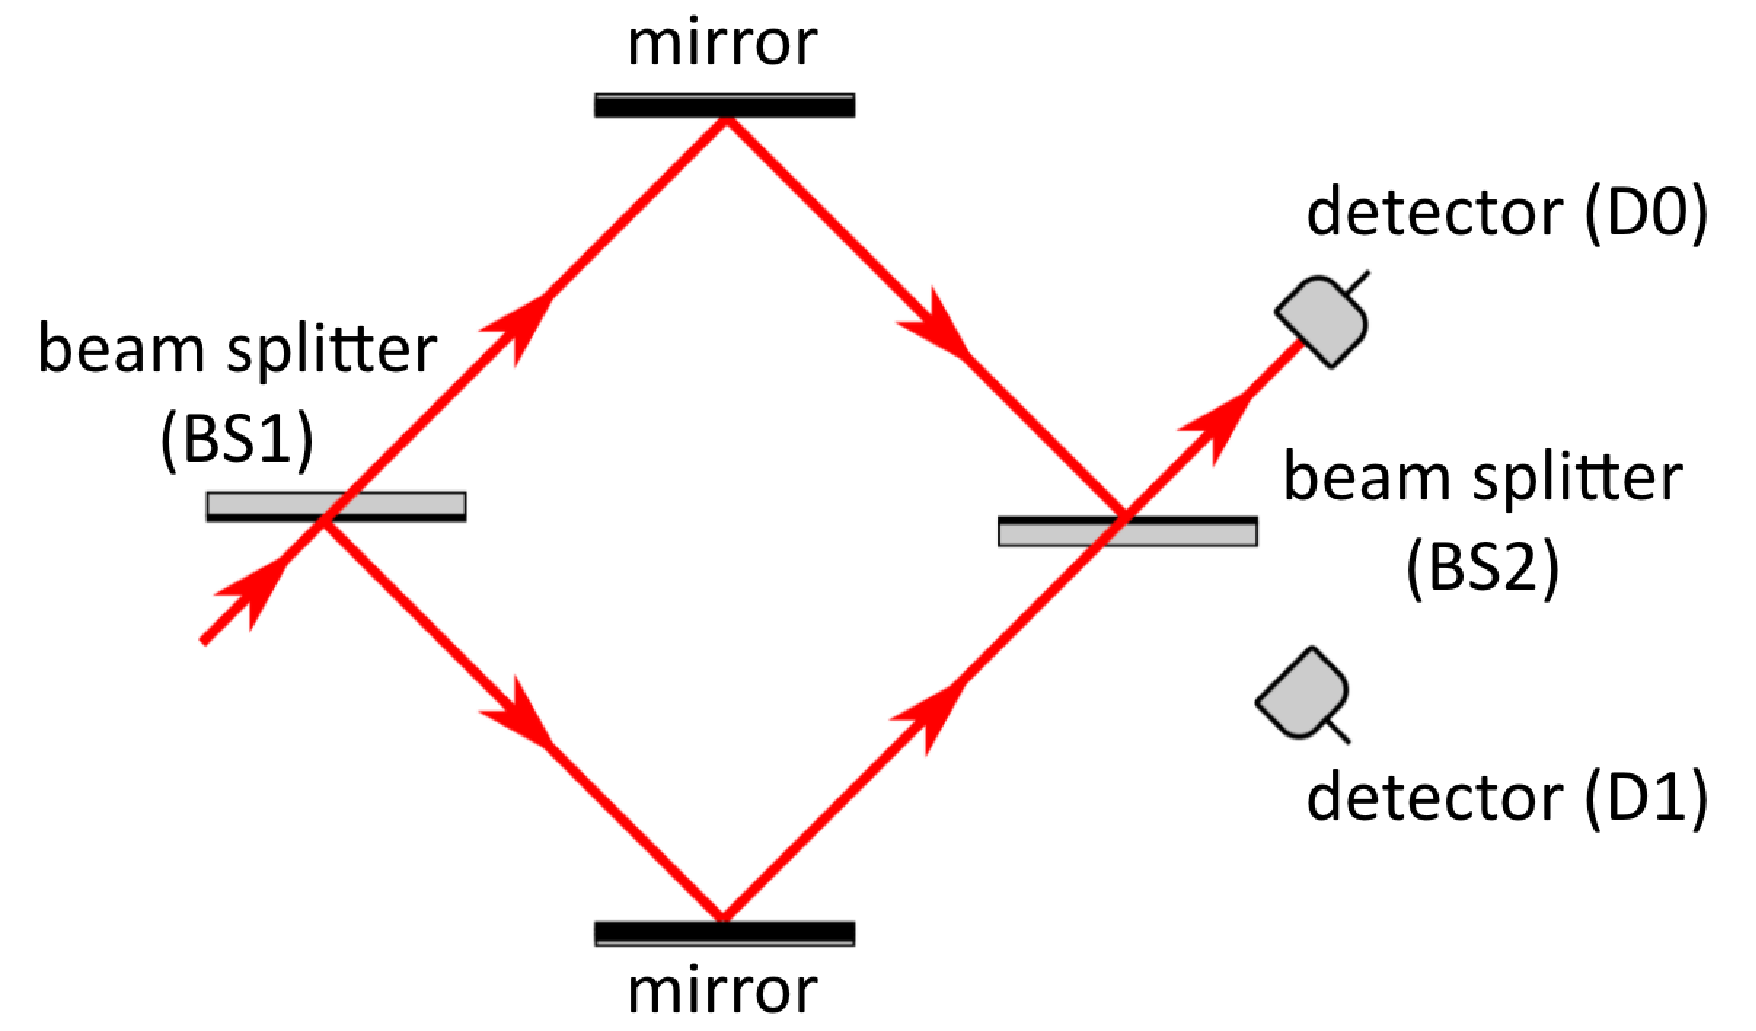
\includegraphics[width=0.8\textwidth]{lesson6/mach_zehnder.pdf}
    \label{fig: 1}
    
        \caption{Mach-Zehnder interferometer.}
    
\end{figure}

% Single photon Mach-Zehnder case
\begin{figure}[H]
   \centering
    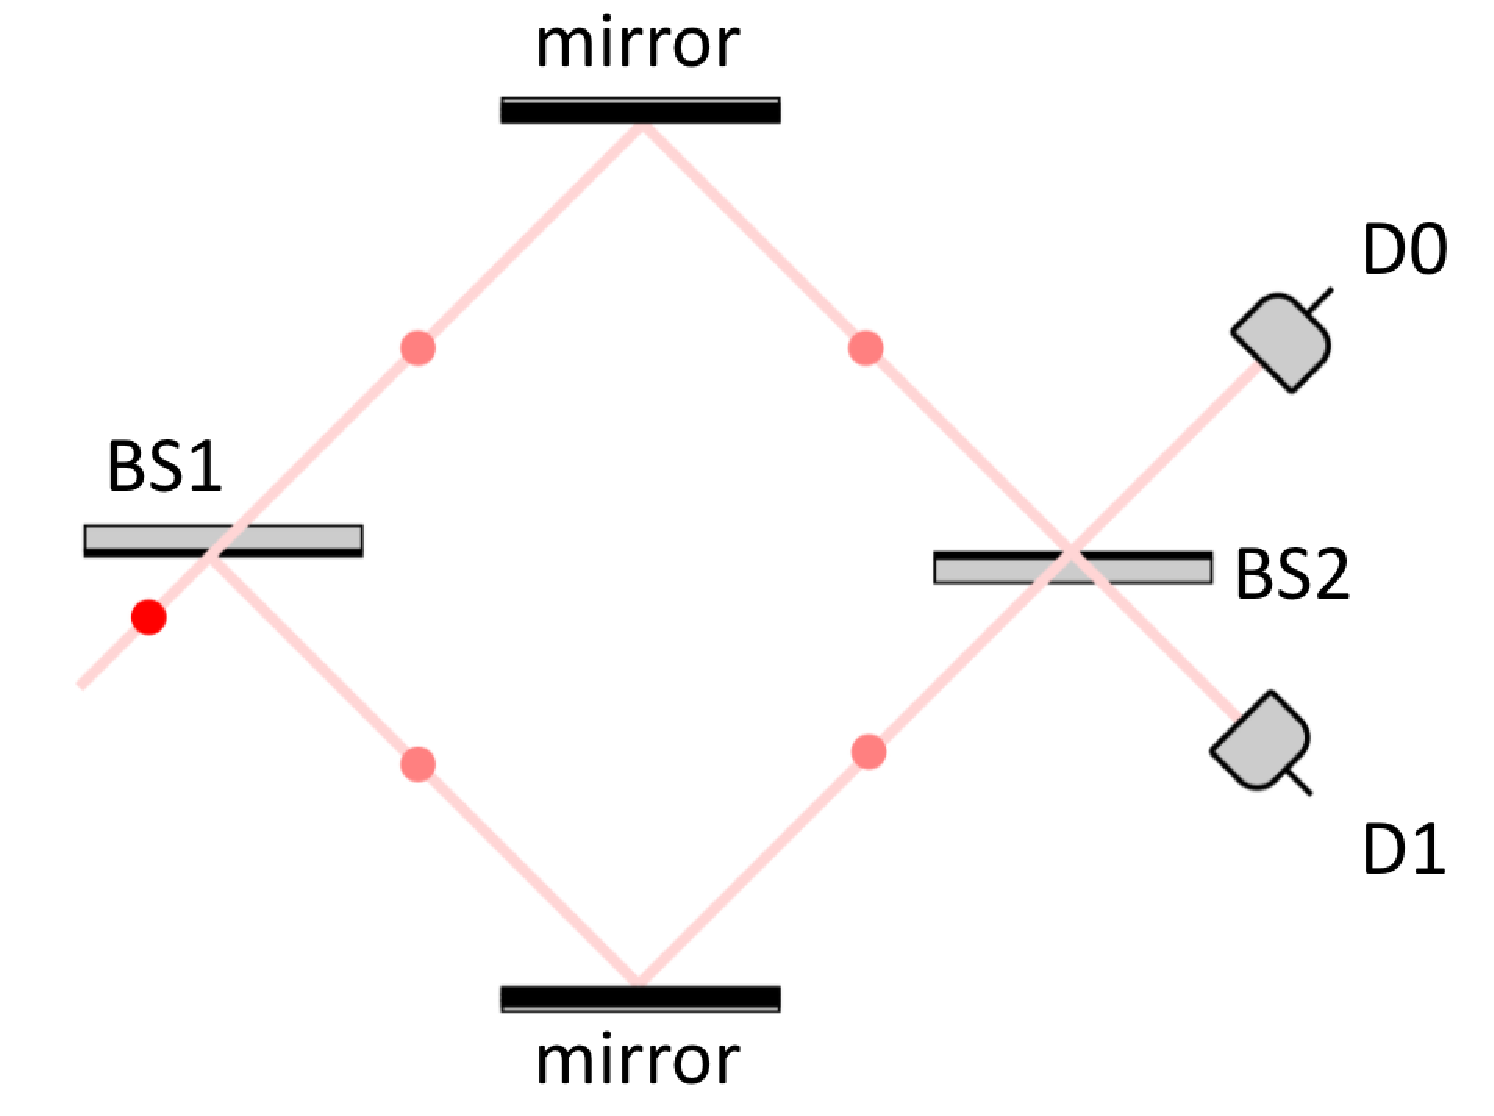
\includegraphics[width=0.8\textwidth]{lesson6/mach_zehnder_single_photon.pdf}
    \label{fig: 1}
    
        \caption{Mach-Zehnder interferometer with a single photon.}
    
\end{figure}

% 0 ket top
\begin{figure}[H]
   \centering
    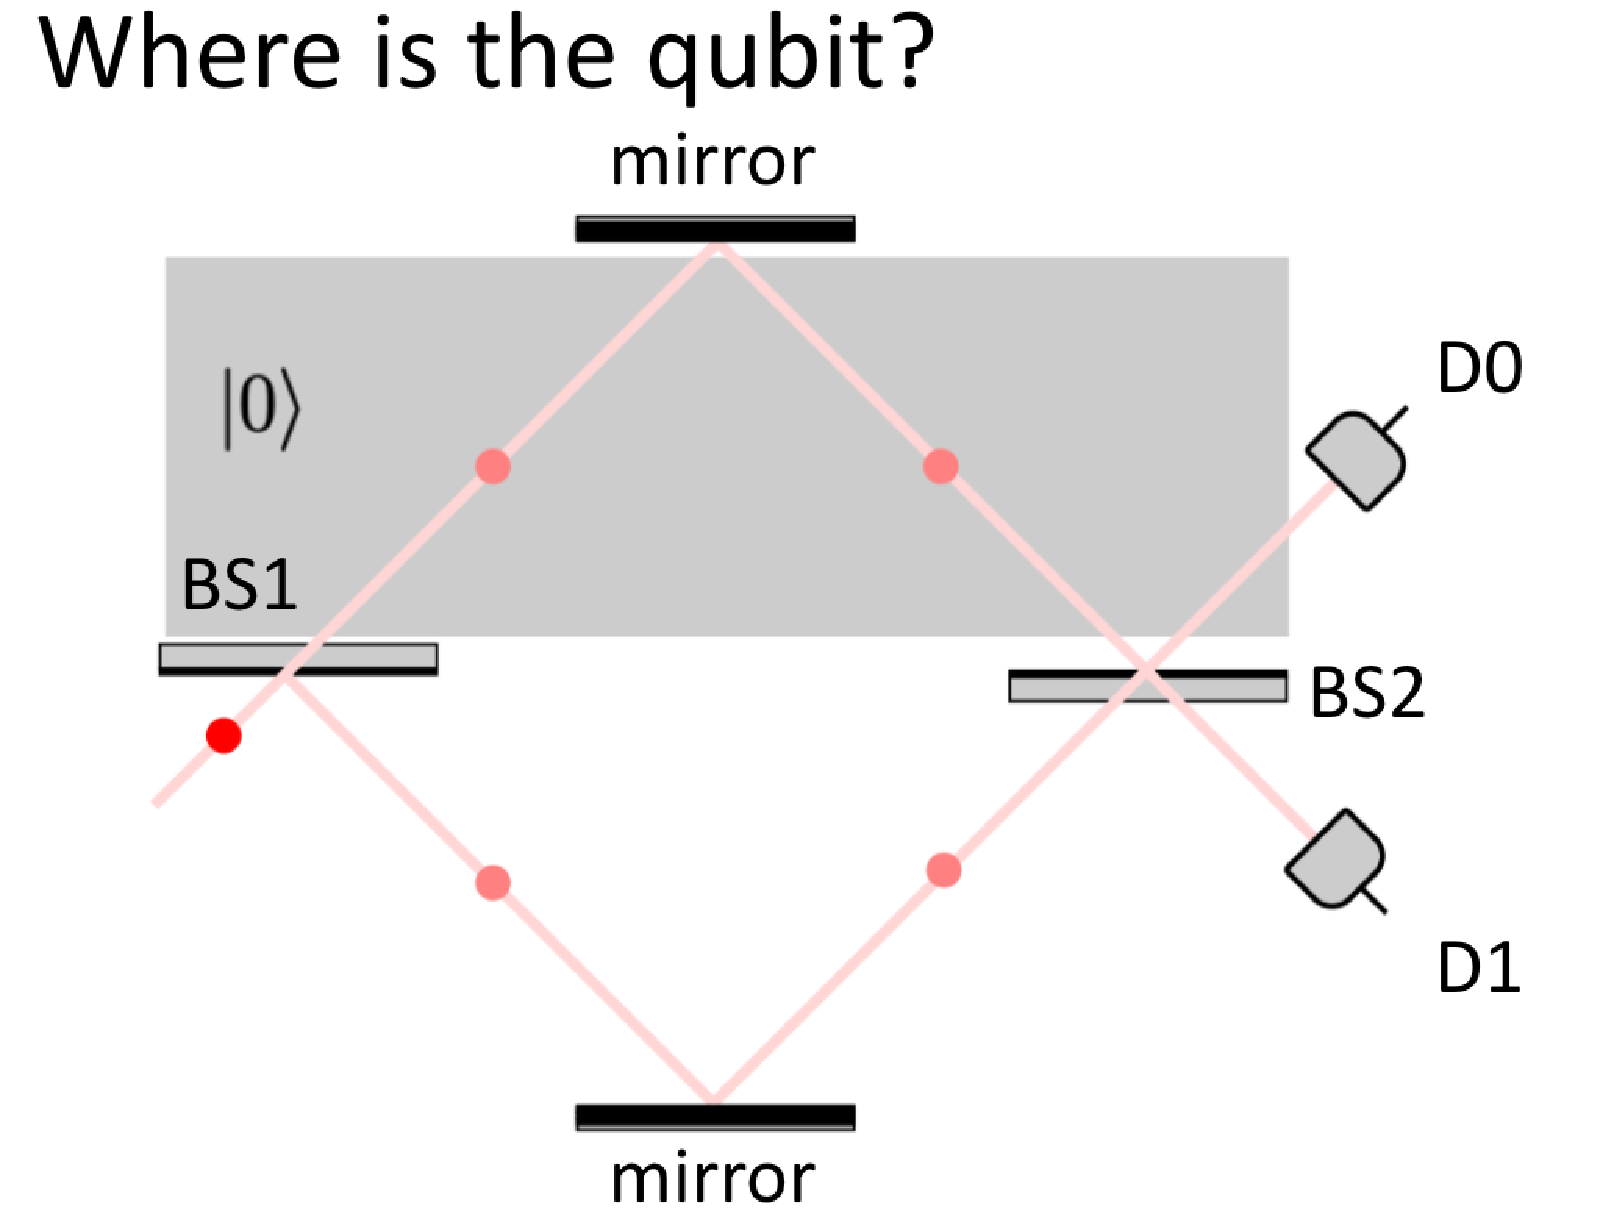
\includegraphics[width=0.8\textwidth]{lesson6/0_ket_botttom.pdf}
    \label{fig: 1}
    
        \caption{$\ket{0}$ state is represented by a photon in the upper path.}
    
\end{figure}

% 1 ket bottom
\begin{figure}[H]
   \centering
    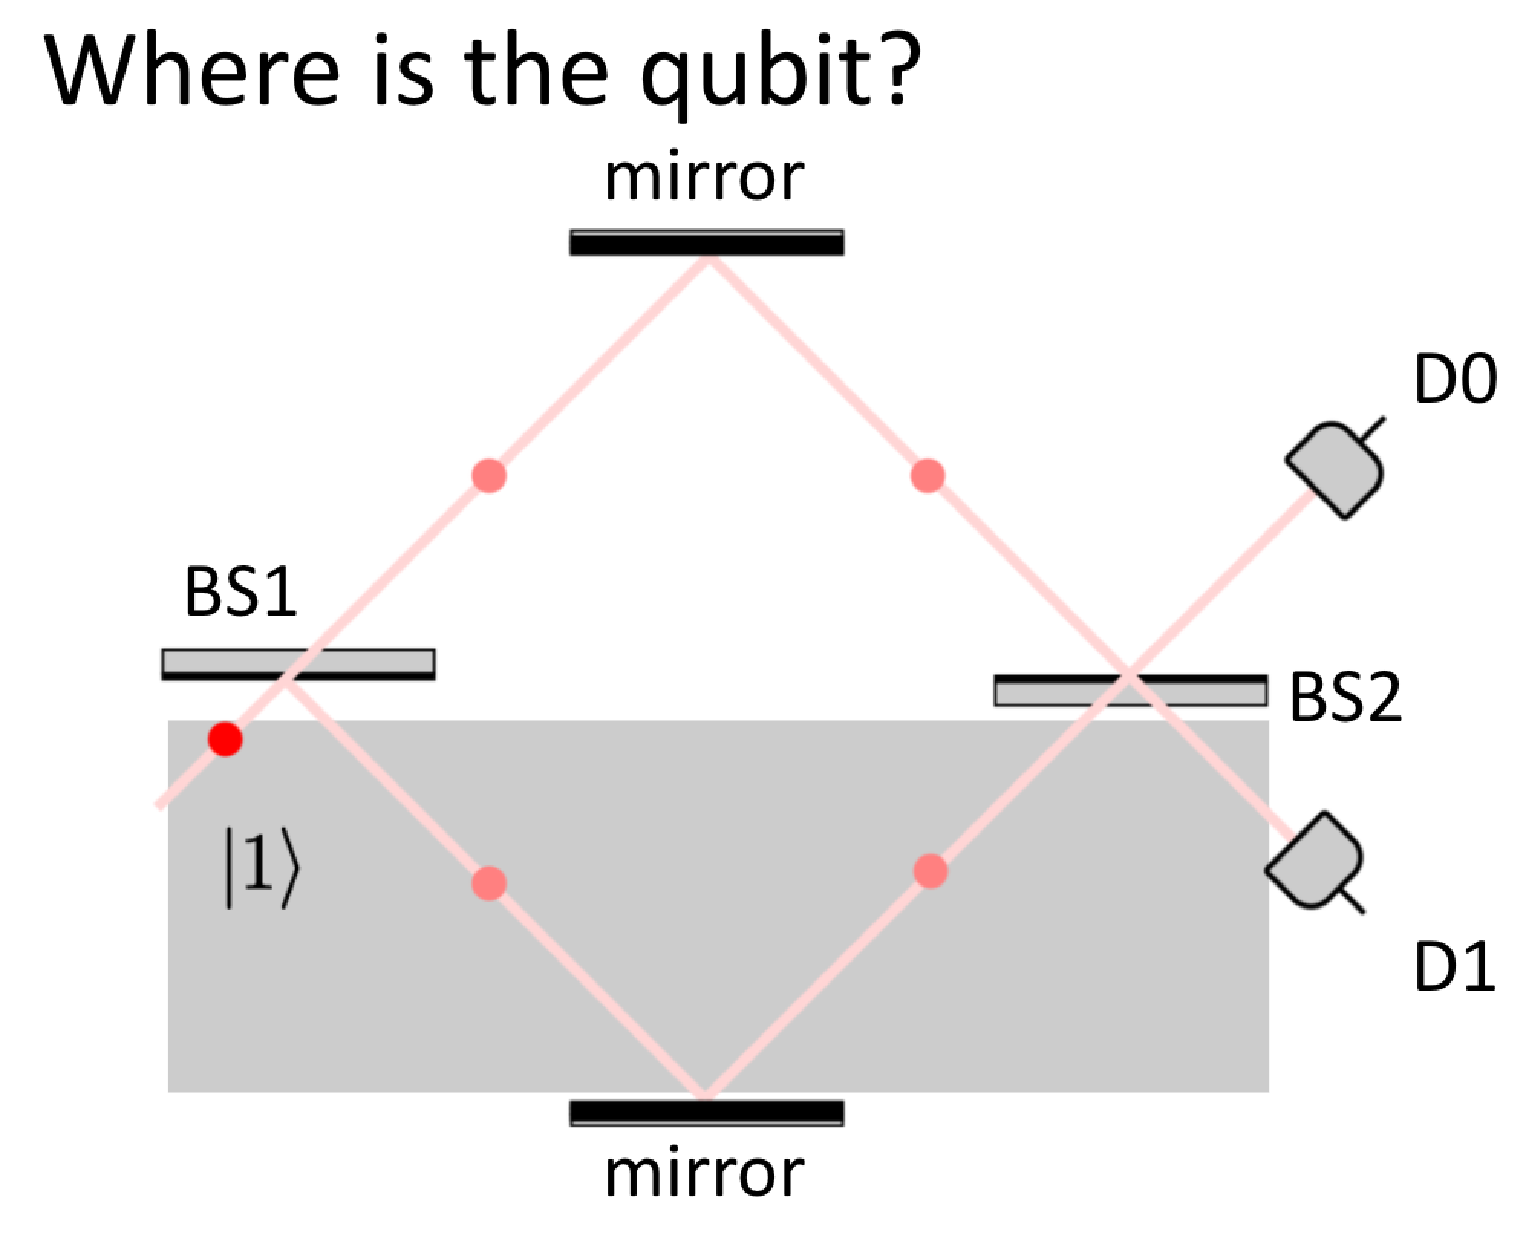
\includegraphics[width=0.8\textwidth]{lesson6/1_ket_bottom.pdf}
    \label{fig: 1}
    
        \caption{$\ket{1}$ state is represented by a photon in the lower path.}
    
\end{figure}

\begin{equation}
B S 2 \cdot B S 1|1\rangle=|0\rangle
\end{equation}

% D0 always clicks
\begin{figure}[H]
   \centering
    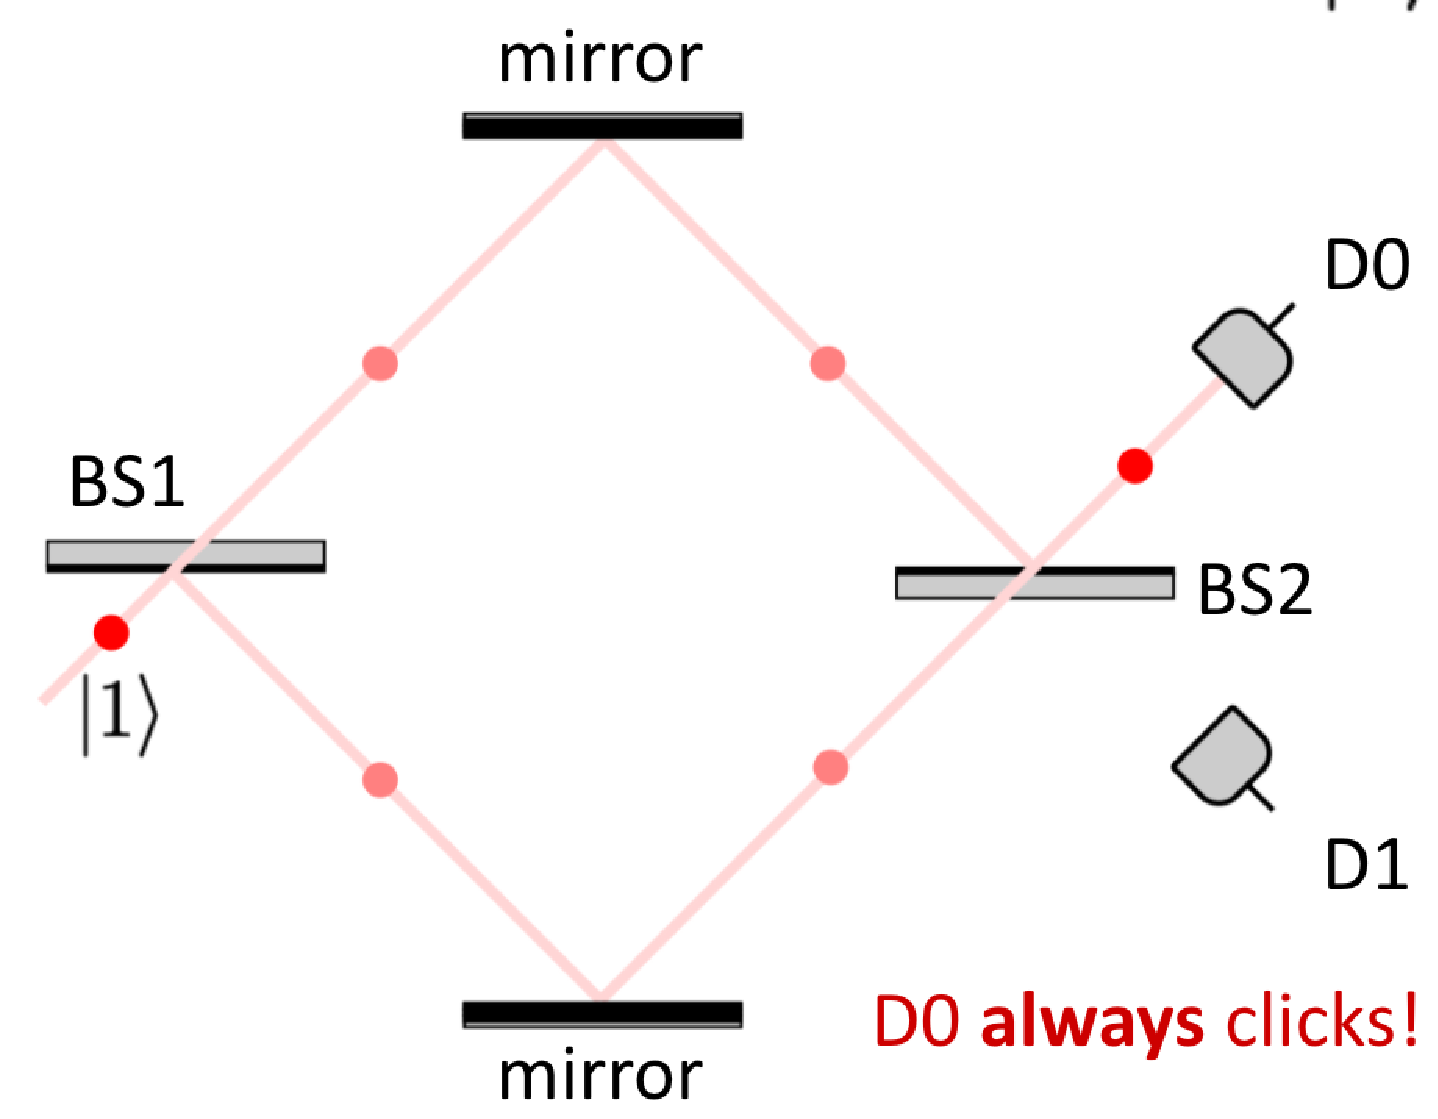
\includegraphics[width=0.8\textwidth]{lesson6/d0_always_clicks.pdf}
    \label{fig: 1}
    
        \caption{$D0$100\% probability.}
    
\end{figure}

% block bottom path
\begin{figure}[H]
   \centering
    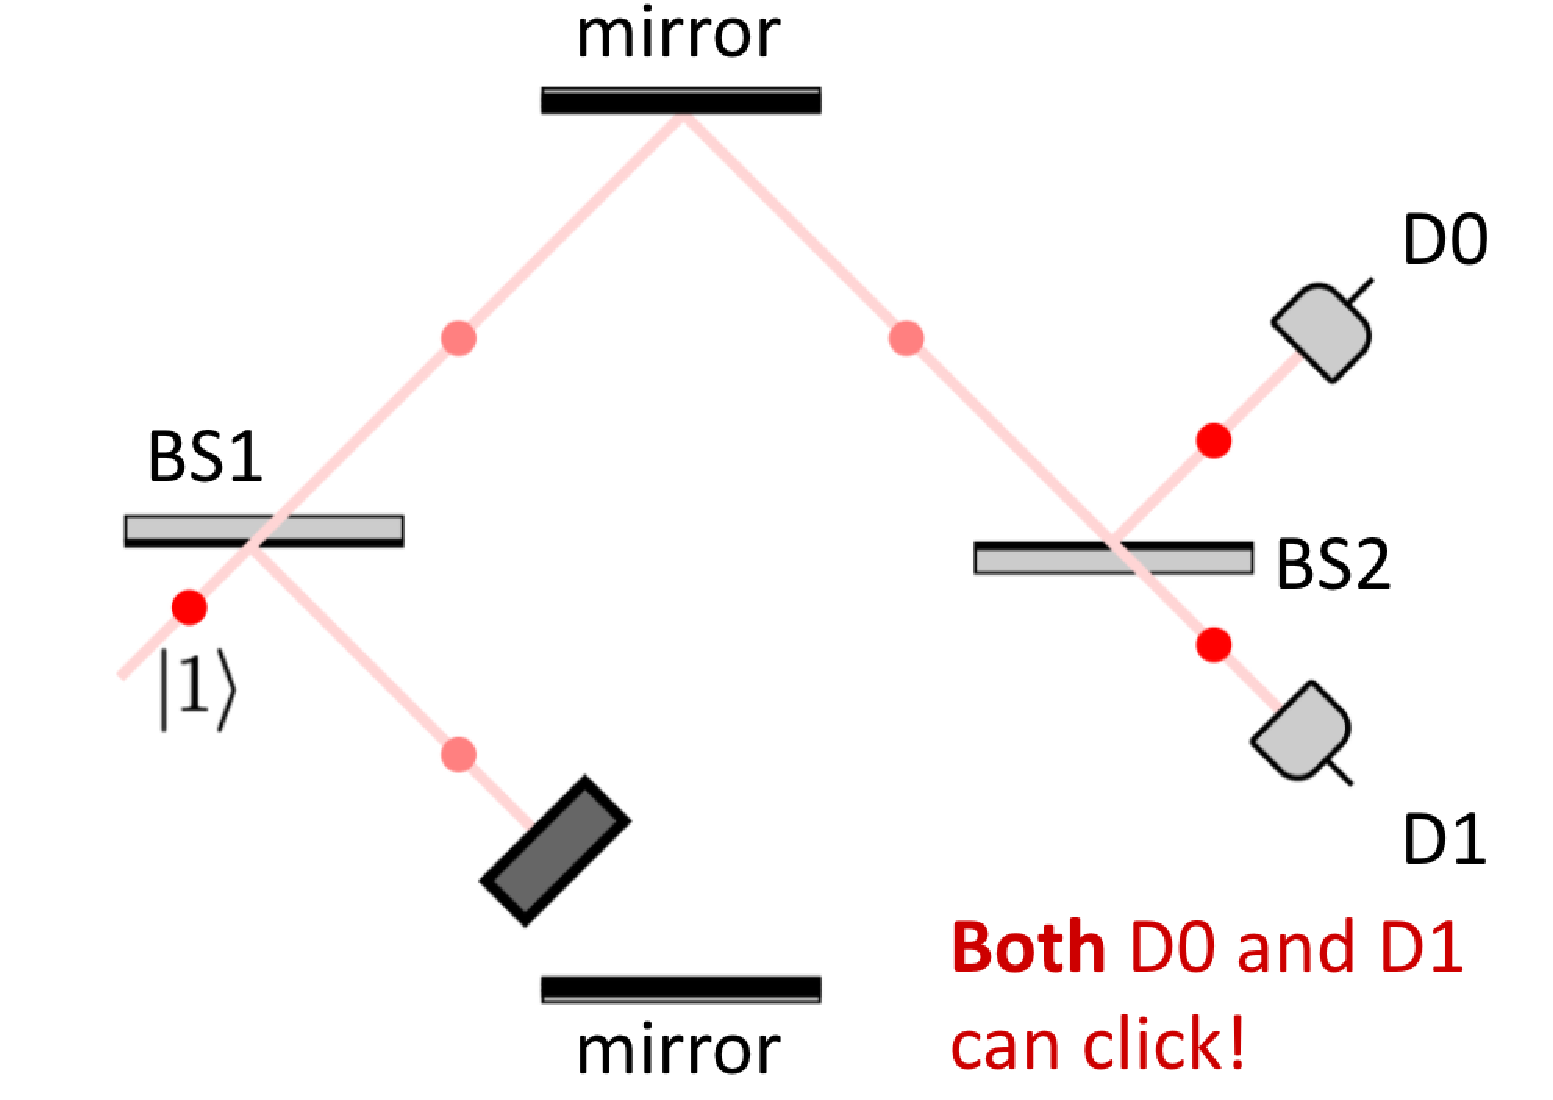
\includegraphics[width=0.8\textwidth]{lesson6/bottom_blocked.pdf}
    \label{fig: 1}
    
        \caption{Lower path blocked.}
    
\end{figure}

Step Four: Interference with Qubits

So, we have seen how light interferes, how waves interfere, and even how single photons interfere. We can in fact, see interference also with single qubits. Let's see how.

Consider that we have a Hadamard gate, and we apply it on the state of a qubit. So we will consider two states (follow pointer)- one is our state zero which is given by this state vector (one zero), another one is (state) one, which is given by its orthogonal friend zero one, and the Hadamard gate is given by this transformation matrix.

If we start in the state zero and apply the Hadamard gate to it, what we get we have seen that already is we get it and we create an equal superposition of state zero and one. Now we can do the same thing again, we can apply another Hadamard gate to this superposition and see what actually happens. Applying the Hadamard to the state zero creates another superposition of zero and one over here, zero plus one. And applying Hadamard gate to the state one creates a superposition of zero and one, but this time with the one having a minus probability amplitude in front of it. So after applications of two Hadamard gates, this is our state (see pointer). You can see that these terms (0+1, 0-1), they both have a positive probability amplitude, plus a half, plus a half. Whereas the other two terms have opposite amplitudes, they've got plus a half, and negative a half. So the effect of that is that the probability amplitudes for ones cancel, whereas the probability amplitudes for the zeros, they constructively interfere, and we end up in a state zero which was our initial state, and this works also for state one if we use that as an initial state, but this time the cancellation of probability amplitudes happens for the zero terms, because they have plus one half minus one half, and the one terms, they constructively interfere because both of them have plus a half, plus a half probability amplitudes. So this may not surprise you too much. After all, applying Hadamard twice actually applies the identity which is doing nothing, that's because the Hadamard gate is its own inverse.

So let's consider different transformations that do not have this property. In particular, let's go consider two transformations. Let's call them BS1 and BS2. You can see that BS1 is actually our previous Hadamard gate but let's just keep calling it BS1 for reasons that will become apparent a little bit later. And this BS2 looks a little bit similar like a Hadamard gate, but this time the minus is not located over here (bottom right), but it's over there (top left). But you can check for yourselves that applying these gates in sequence is not the same thing as doing nothing. In particular, BS2 times BS1 is not equal to the identity. But let's see what happens. Again, we take our initial state. Let's say our initial state is one. We first apply the transformation BS1, and what we get is the following: we apply the Hadamard gate to the vector (zero one), and after simple multiplication we got the following state vector, which is just a superposition of zero minus one. And then, we continue applying our gates. This time, we apply BS2, and what we get is in fact another translation. You see, over here (see pointer), the probability amplitudes corresponding to state zero, they constructively interfere, whereas the probability amplitudes contributing towards state one, they destructively interfere, and therefore the probability amplitude for state one becomes zero. This minus term that appears here is not important, it has no consequence because it's just a global phase, so we can just ignore it.

Now, let's consider an optical instrument called a Mach-Zehnder Interferometer. It consists of two beam splitters which are BS1 and BS2, and two mirrors over here and over here (follow pointer), and two detectors, and the games that we like to play with this Mach-Zehnder Interferometer is that we feed in some light into the first beam splitter, and then we ask the questions when will D0 click, when will detector D1 click, what's the intensity measured detector D0, was the intensity measured at detected D1, and so on. In this particular case, we assume that we only have light coming in from the bottom over here (follow pointer), and the mirrors and beam splitters are set in such a way that the path lengths are the same. Here (follow pointer), what can happen is the light can be reflected from the first beam splitter, bounce off the mirror, and enter the second beam splitter, or it can be transmitted through the first beam splitter, bounce off the top mirror, hit the second beam splitter interfere with the beam coming from the bottom branch, and either it will be detected at D0 and D1. If the path lengths are the same, then for this scenario, it will always be detected in this top detector D0.

Now, let's consider that we have again only a single photon entering our Mach-Zehnder Interferometer, and then again, the single photon can be reflected at the first one or transmitted. It bounces off the mirrors which don't really do anything, they just alter the path of the photon and then it recombines at the second beam splitter, and we ask the question: does it get detected at D0 or does it get detected at D1?

Also, the Mach-Zehnder Interferometer implements our qubit. How? Where is the qubit? Well, if the photon is found in the top half of the interferometer, we say that it's in the state zero. On the other hand if it's found in the bottom half, we say that it's in the state one. So here the different paths encode different computational states of the qubit.

So let's consider our initial state to be in state one, meaning it enters our Mach-Zehnder Interferometer from the bottom half.

And in fact, now you see why we have called those previous transformations BS1 and BS2. They correspond to the mathematical description of how these beam splitters affect the probability amplitudes of our qubit. And, we proved before that if we first act on our qubit, on our initial state, with beam splitter one, and subsequently with beam splitter two, then we know that if the initial state is in the bottom half, then the output state will always be found in the top half, meaning D0 detector always clicks. But yet again, the situation is very similar to the previous step. Here, there is only a single photon found in the Mach-Zehnder Interferometer, and we cannot divide photons, there's always just one, yet somehow it knows that it has to interfere with itself and always goes towards a detector D0. Now, let's do a simple test. Let's actually put some absorbing material and block the possibility of the photon going through the lower half of the Mach-Zehnder Interferometer. What do we see? Well, the photon coming in here can get reflected. If it does get reflected, then it just gets absorbed and we don't get any clicks. However, if it gets transmitted and it goes through, it bounces off the mirror and it is incident onto the second beam splitter, where again, it has an equal probability of being reflected or passing through the beam splitter. Therefore, it has a probability of being detected by both detector D0 and the detector D1. So what we have effectively done by blocking this path of photon in the bottom of the Mach-Zehnder Interferometer is we have prevented interference from taking place at beam splitter two. That is why we see both possibilities D0 and D1.


\newpage
\begin{exercises}

\exer{Write some code to reproduce the static plot in Fig.~\ref{fig:decaying-superposition}.  Try to make your code represent the equations as nearly exactly as possible.  The plots and animations in our course were created using the Python package {\tt manim}, but your instructor may have different instructions for you.}

\exer{Write some code to reproduce the animated plot in Fig.~\ref{fig:propagating-waves}.  Try to make your code represent the equations as nearly exactly as possible.  The plots and animations in our course were created using the Python package {\tt manim}, but your instructor may have different instructions for you.}

\end{exercises}

